% Chapter 04: Data Description and Analysis

\section{Data Description}

% Chapter 04 / Grid Resolution and Patch Size Study

The problem was first set up to match the experimental installation so that the incoming boundary layer profiles would match, as shown in \Cref{fig:tun}. Slip wall boundary conditions were applied inside the plenum for simplicity and a specified pressure boundary condition was applied at the patch to model air being drawn out of the plenum by a suction pipe.

\figSmallPatch
\figMeshOverlay

%\begin{figure}[H] \centering
%\begin{subfigure}{.8\textwidth} \centering
%  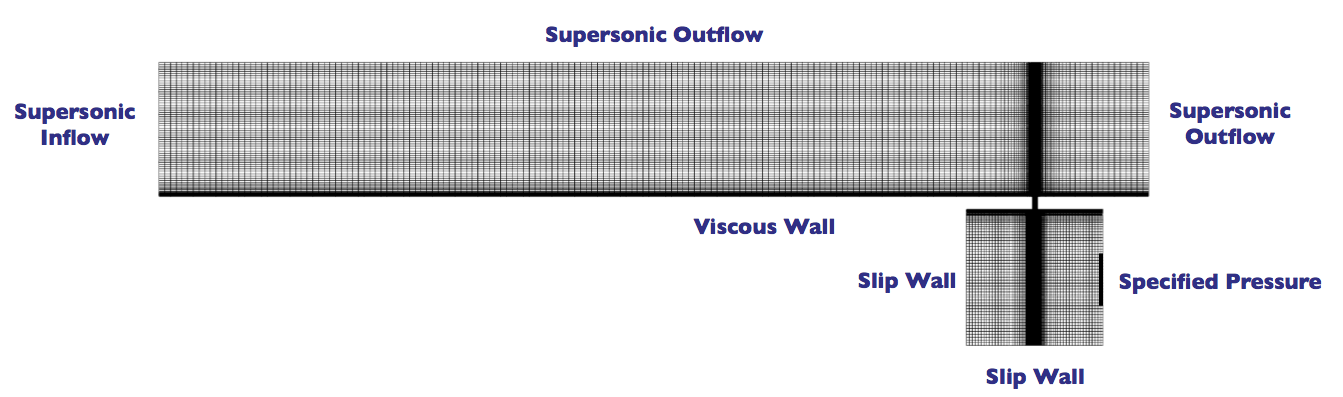
\includegraphics[width=1\linewidth]{mesh.png}
%\end{subfigure}
%\begin{subfigure}{.65\textwidth} \centering
%  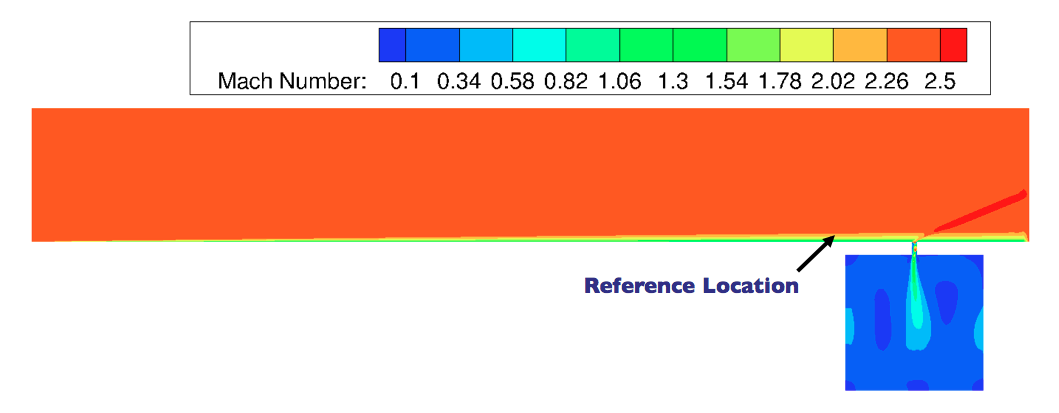
\includegraphics[width=1\linewidth]{overview_solution.png}
%\end{subfigure}%
%  \caption{Grid setup}
%  \label{fig:tun}
%\end{figure}

For the grid resolution study, grid spacing in the hole and plenum was varied relative to the diameter of the bleed hole to create three grids, each one twice as refined as the previous as shown in \Cref{tab:grid}. The resulting mesh can be seen in \verb|$figgrid_patch$|. The patch size was also varied to examine its effect on the recirculation in the plenum. Three different patch sizes were also examined against each of the grid refinement levels, where each patch size was double the previous length. This resulted in 9 cases between the three different grid refinements and patch sizes.

%\tabTestMatrix

%\begin{figure}[H] \centering
%  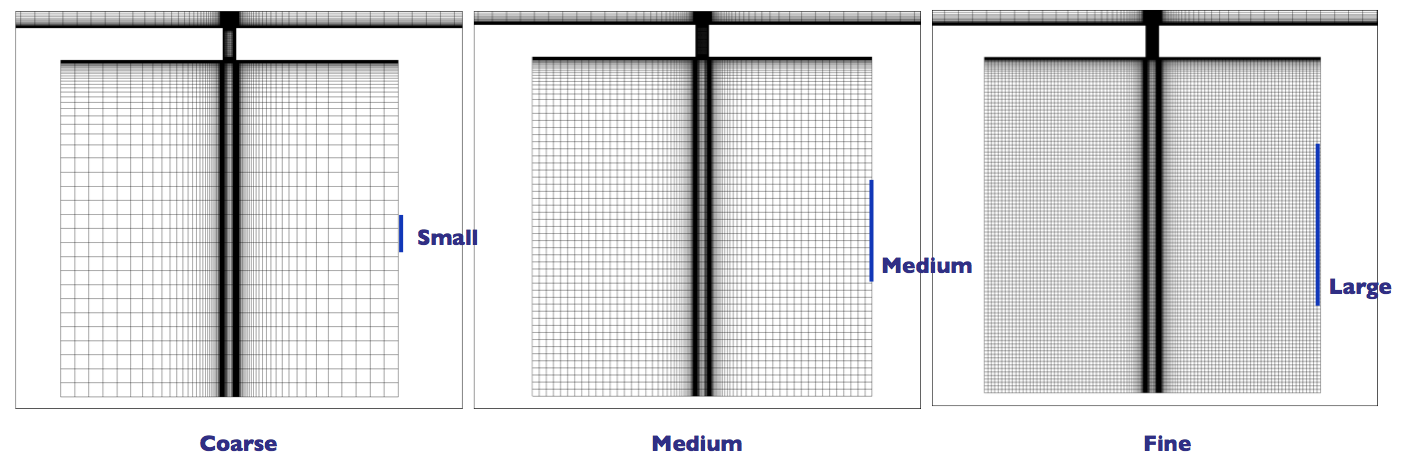
\includegraphics[width=.98\linewidth]{grid_size.png}
%  \caption{Grid spacing in the plenum with the patch sizing overlaid.}
%  \label{fig:grid_patch}
%\end{figure}

The results of the grid resolution study and the patch size study in \verb|fig:small,fig:med,fig:large| and summarized in \verb|fig:massflow_results| show that using a pressure boundary condition can produce recirculation on the boundary, especially for the large patch. This is not believed to be physical and is also undesirable since it produces extra recirculation. This observation led to using a suction pipe grid to draw the air instead of using a pressure boundary condition. This also showed that conservation of mass in the plenum was not well conserved if the grid was not fine enough. The massflow through the hole between all the cases were all consistent with one another, but the massflow out the plenum (suction pipe) can vary significantly from the massflow into the plenum (hole). \verb|fig:massflow_results| illustrates this inconsistency where red squares represent a difference greater than 10\% between plenum outflow and plenum inflow, yellow squares represent a difference of 10\% or less between plenum outflow and plenum inflow, and green squares represent a difference of less than 3\% between plenum outflow and plenum inflow.

%\begin{figure}[H] \centering
%\begin{subfigure}{.33\textwidth} \centering
%  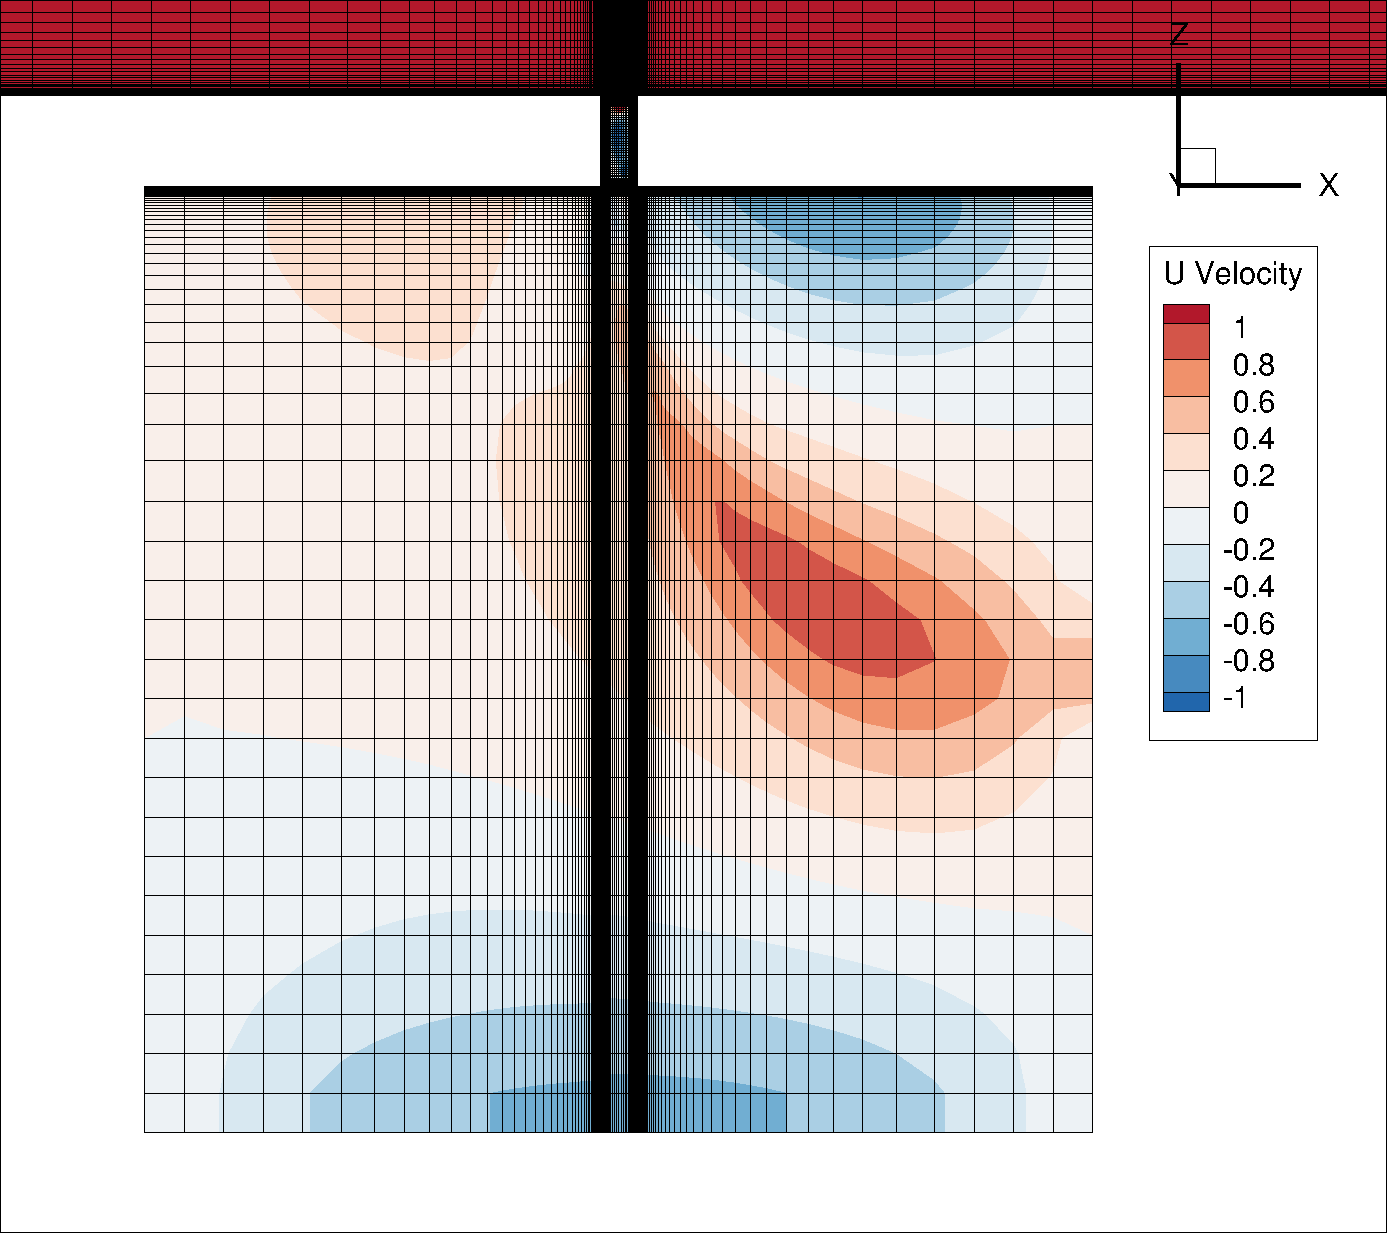
\includegraphics[width=1\linewidth]{1-1_grid.png}
%\end{subfigure}%
%\begin{subfigure}{.33\textwidth} \centering
%  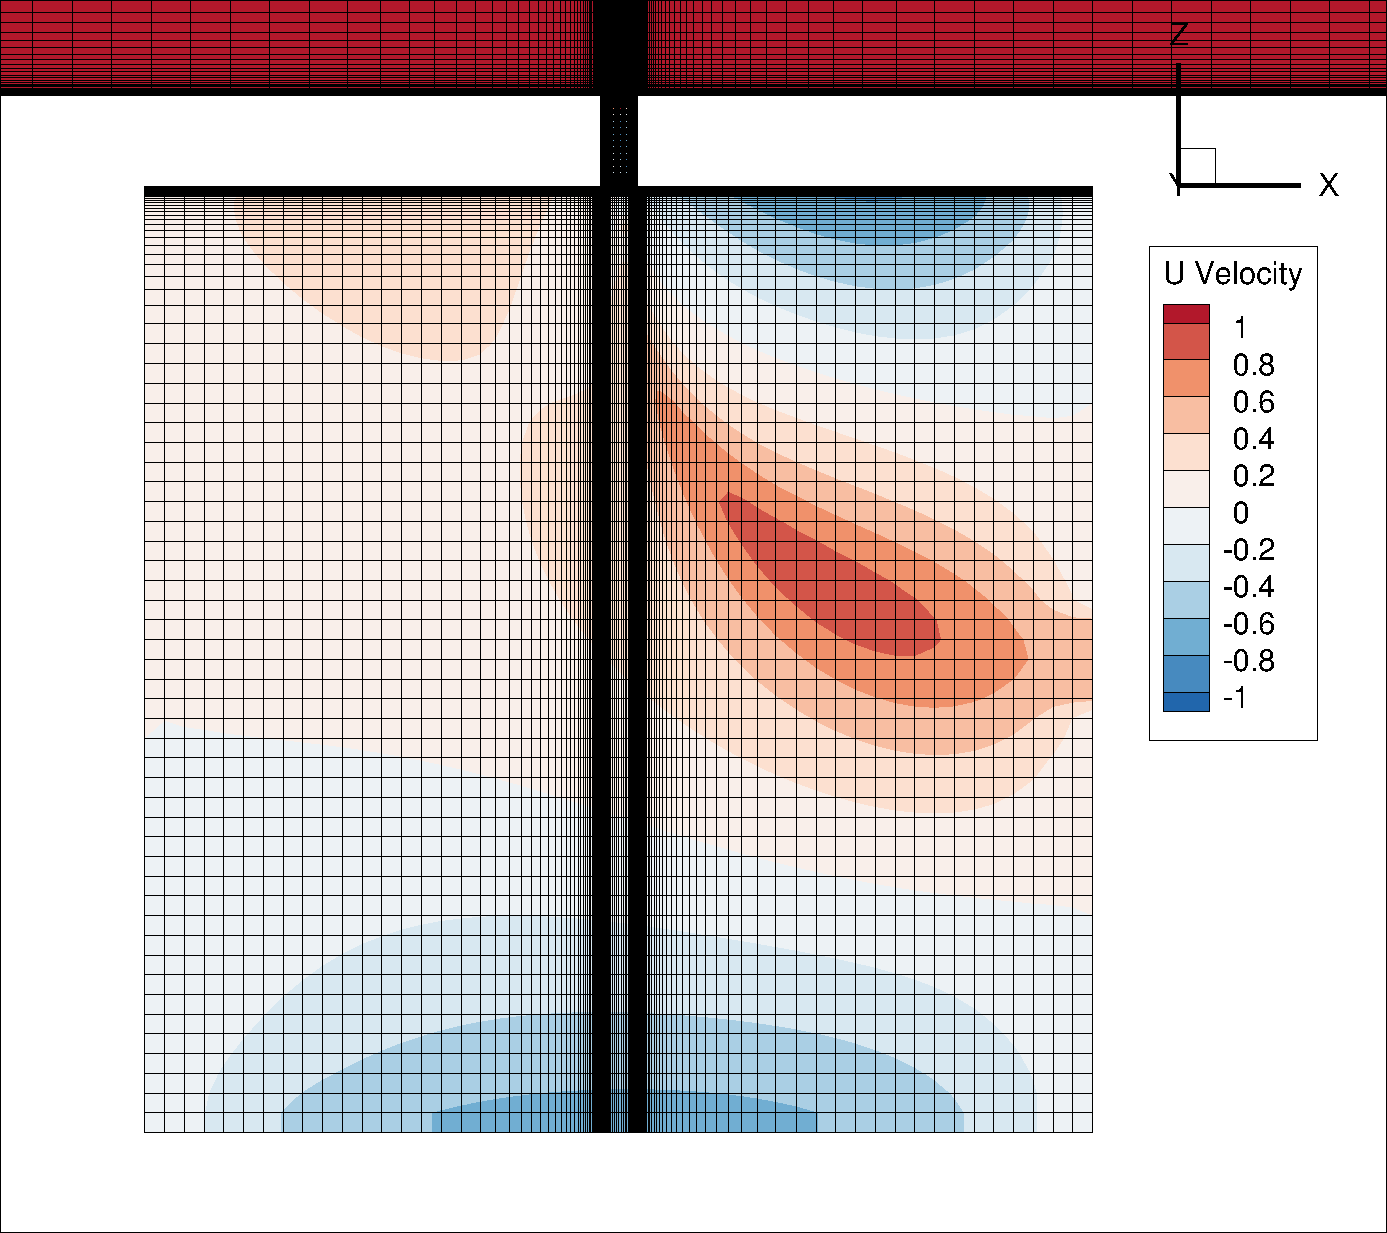
\includegraphics[width=1\linewidth]{1-2_grid.png}
%\end{subfigure}%
%\begin{subfigure}{.33\textwidth} \centering
%  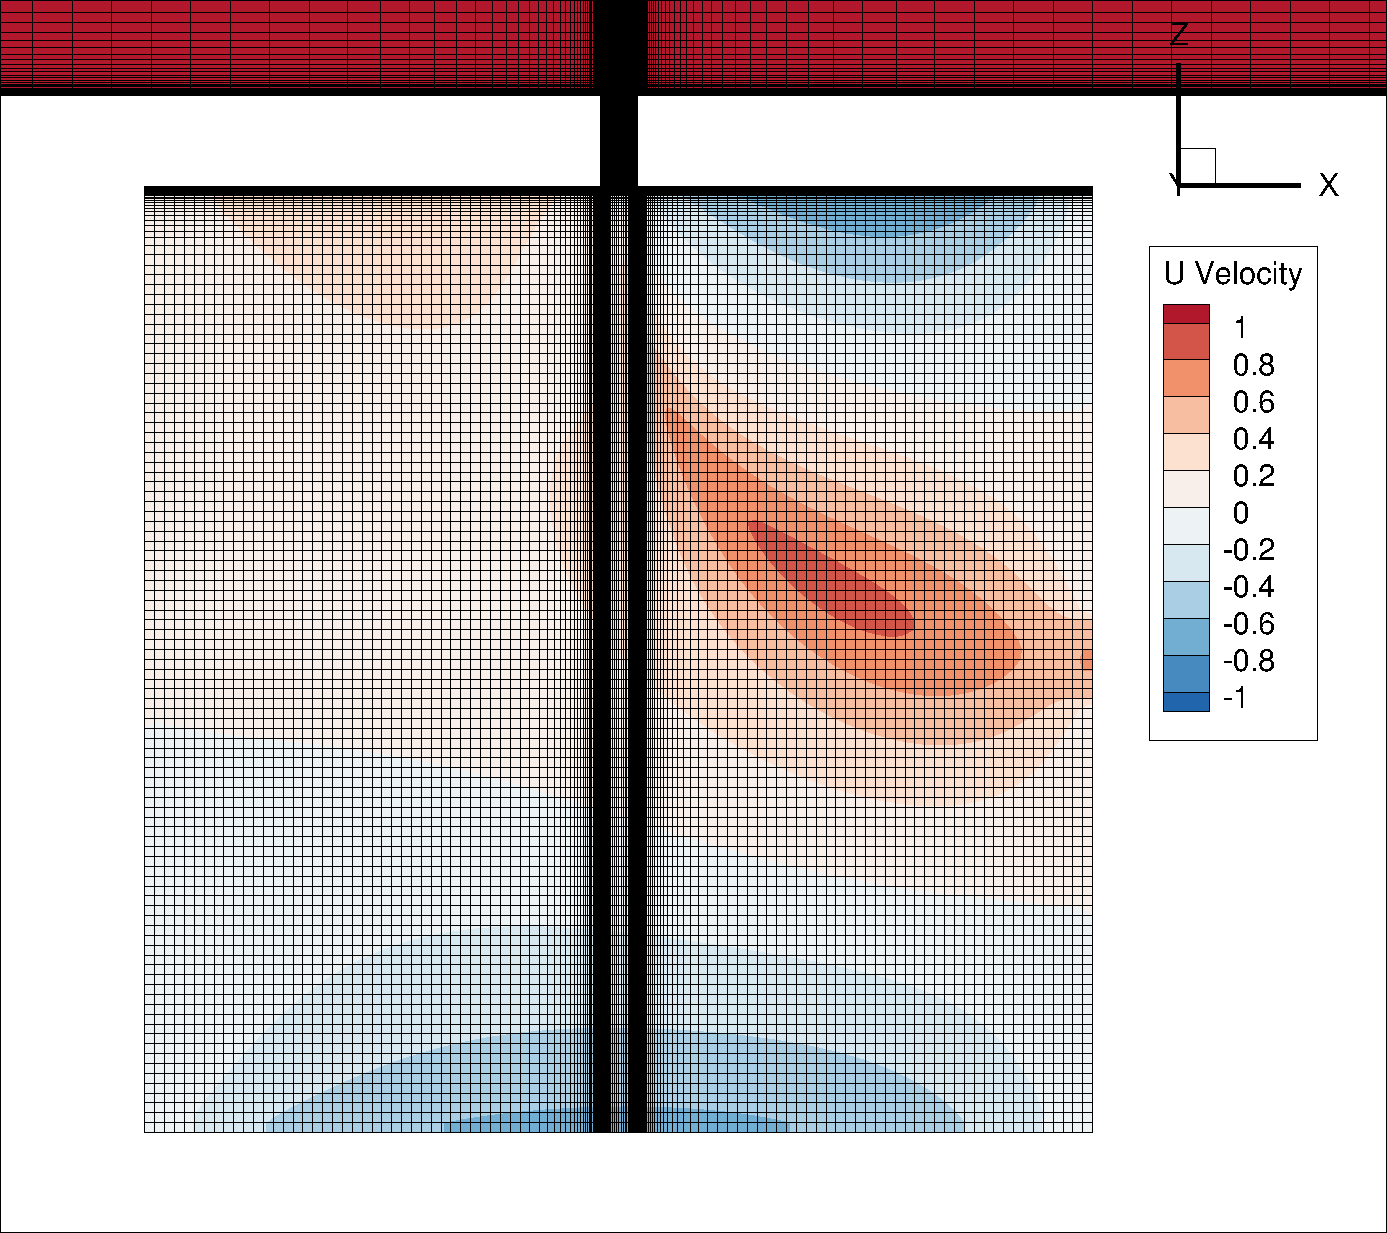
\includegraphics[width=1\linewidth]{1-3_grid.png}
%\end{subfigure}
%\begin{subfigure}{.33\textwidth} \centering
%  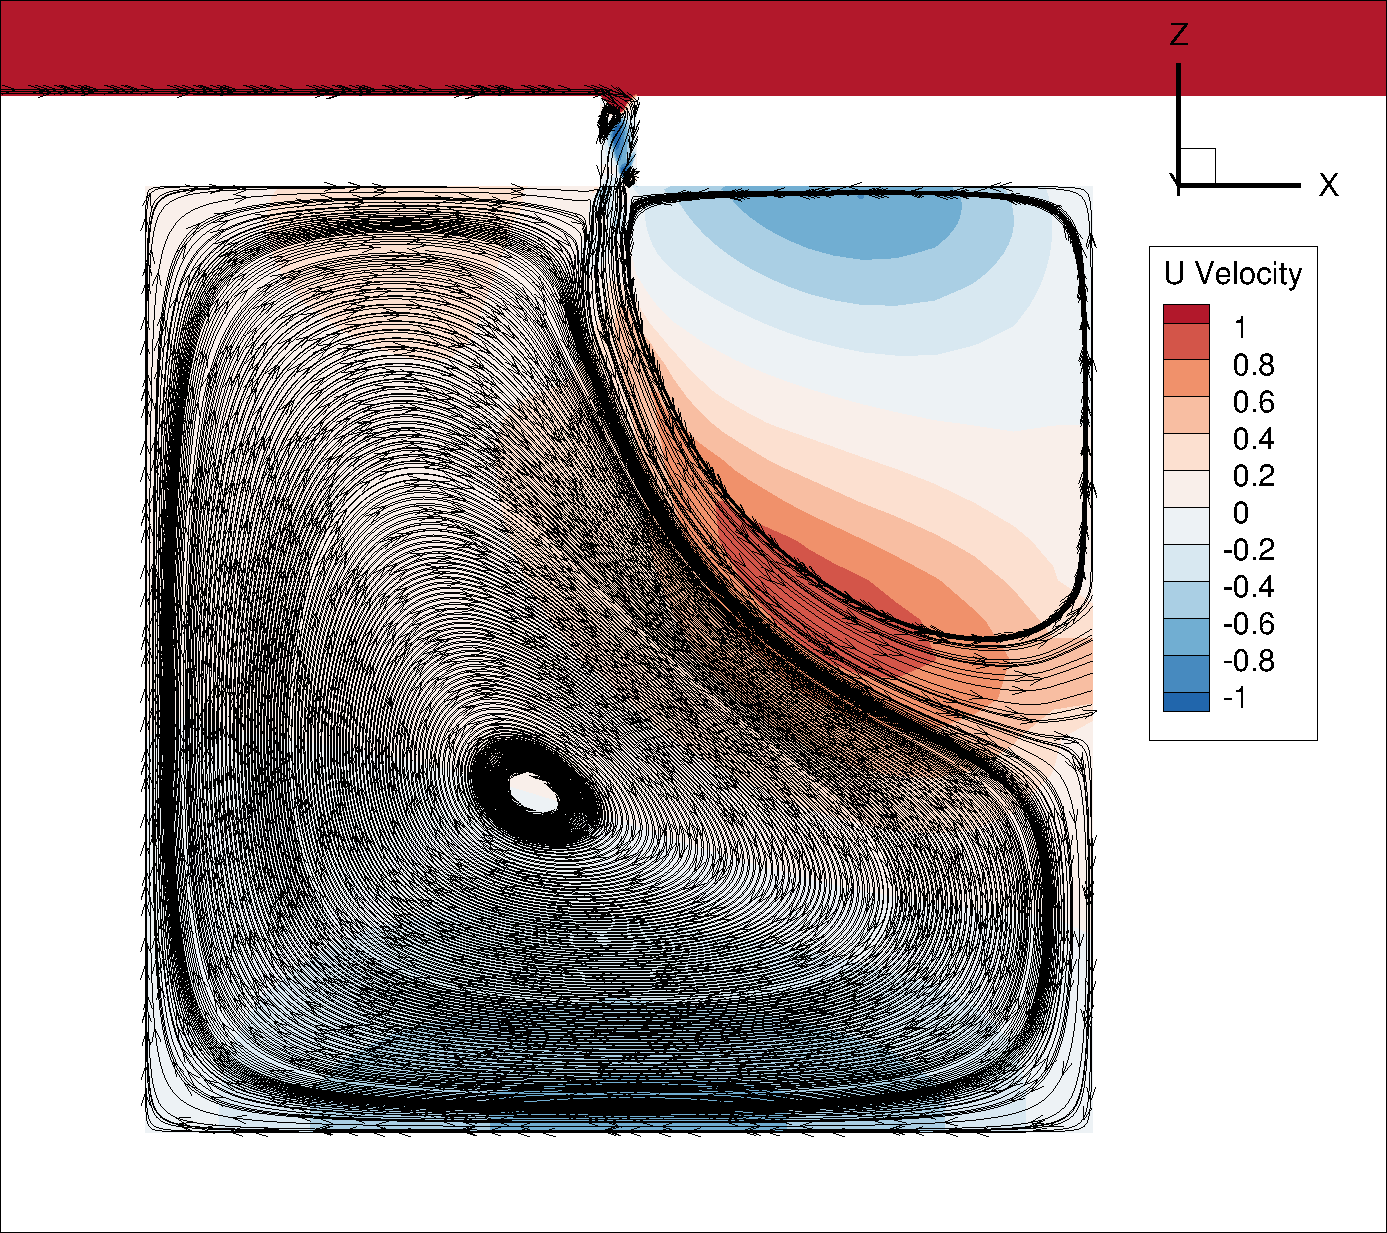
\includegraphics[width=1\linewidth]{1-1_streamlines.png}
%\end{subfigure}%
%\begin{subfigure}{.33\textwidth} \centering
%  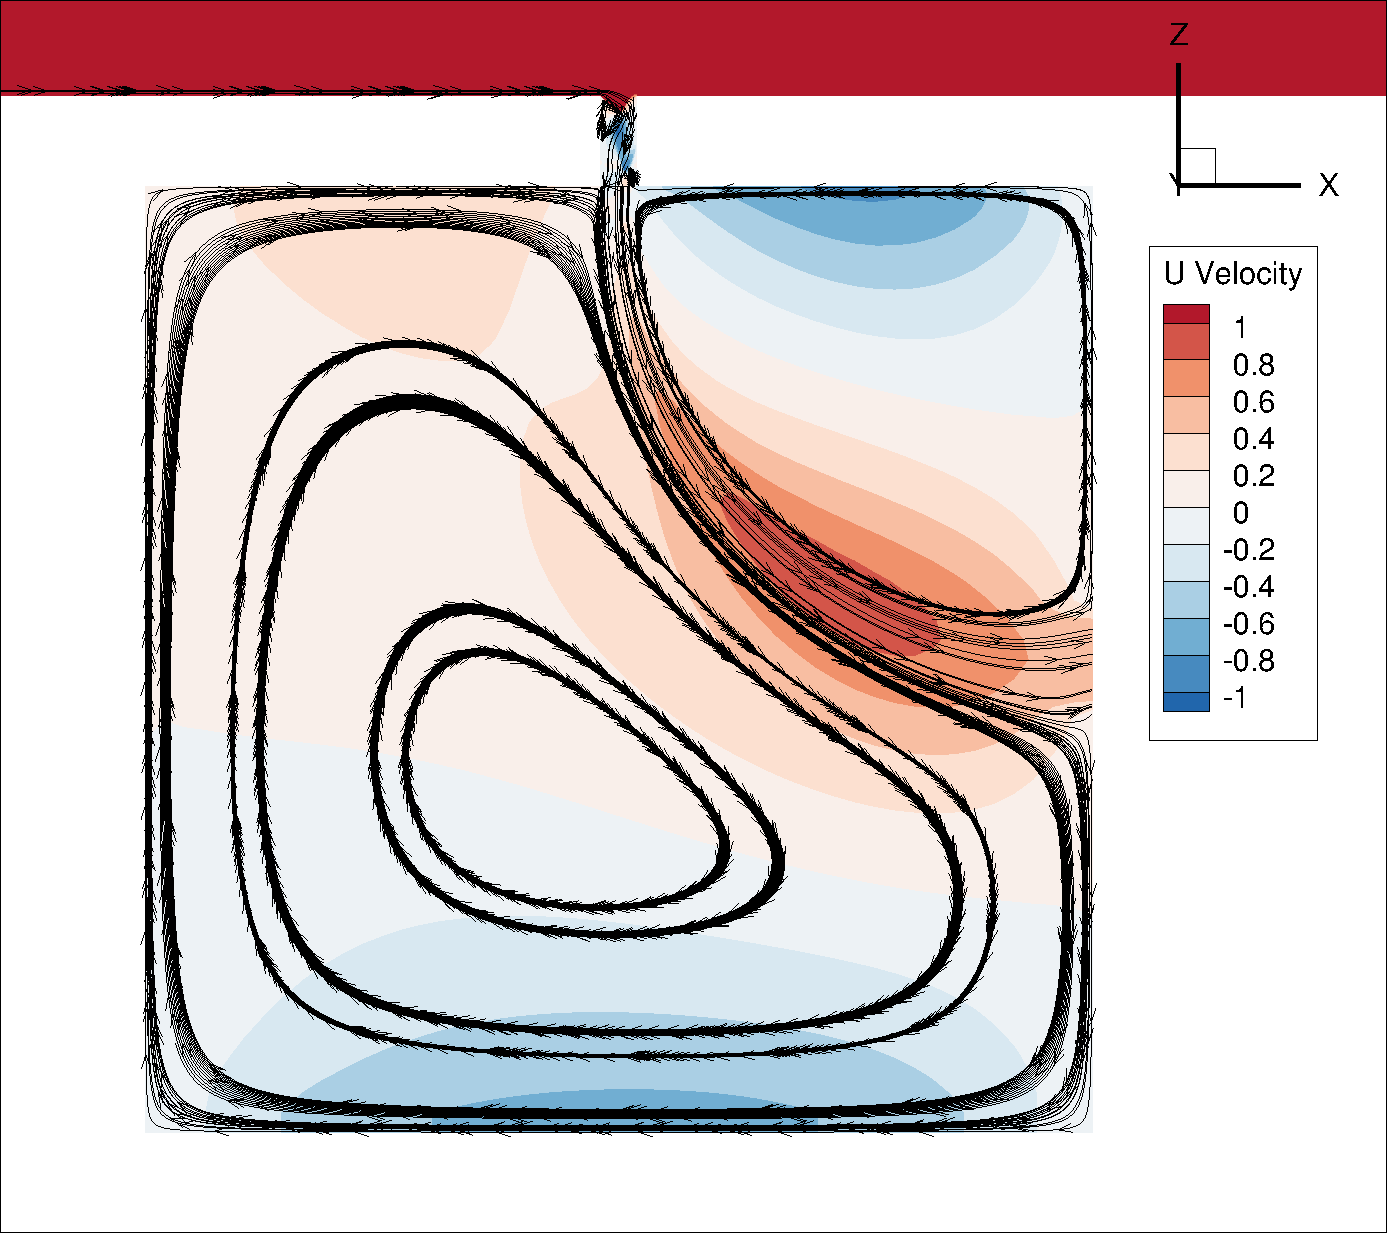
\includegraphics[width=1\linewidth]{1-2_streamlines.png}
%\end{subfigure}%
%\begin{subfigure}{.33\textwidth} \centering
%  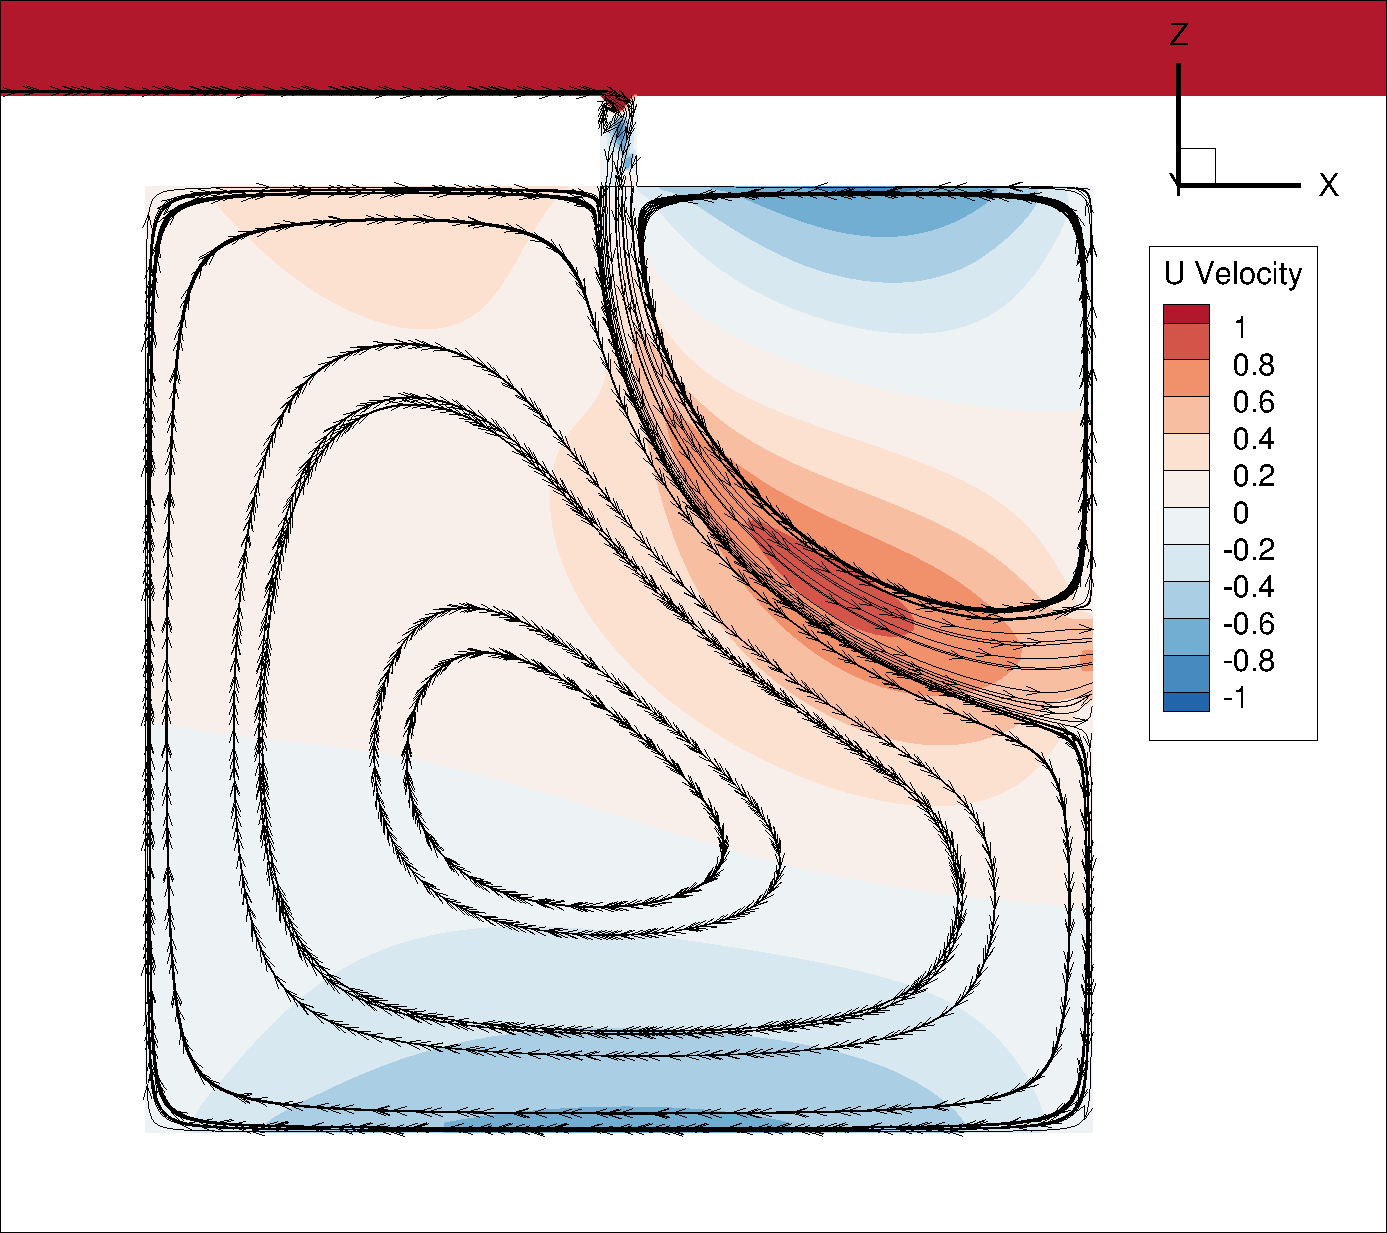
\includegraphics[width=1\linewidth]{1-3_streamlines.png}
%\end{subfigure}
%  \caption{Grid resolution study of the contours of u-velocity and streamlines for the small patch}
%  \label{fig:small}
%\end{figure}

%\begin{figure}[H] \centering
%\begin{subfigure}{.33\textwidth} \centering
%  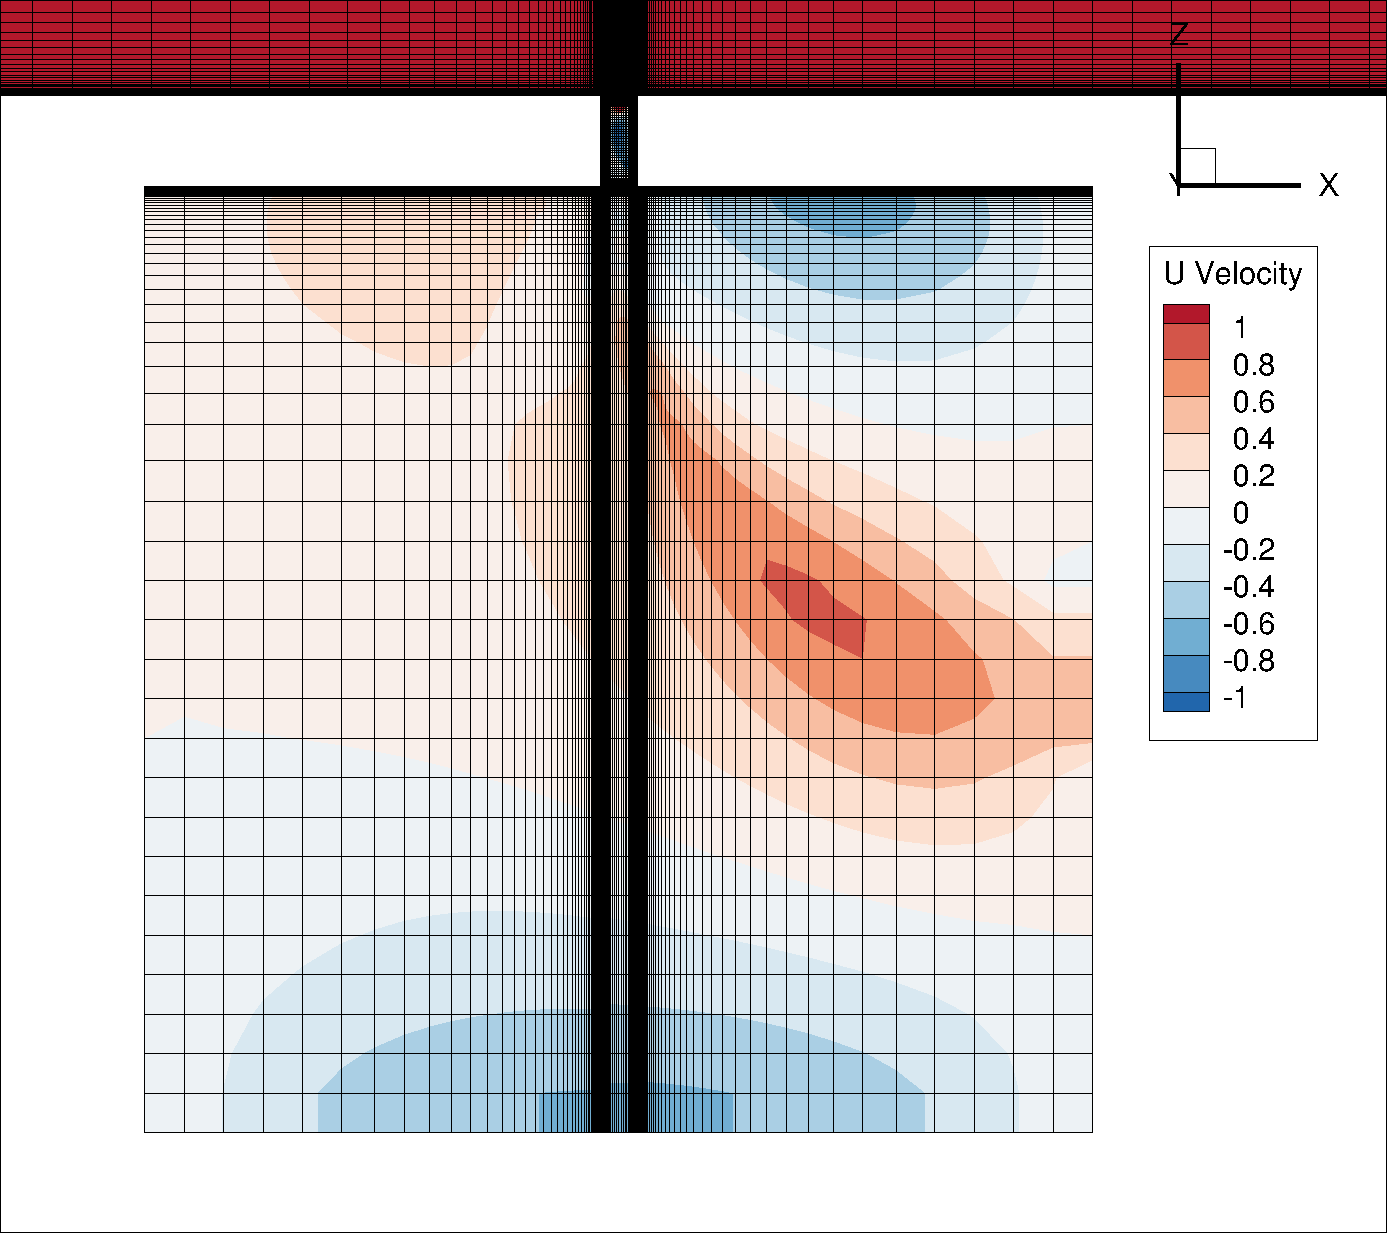
\includegraphics[width=1\linewidth]{2-1_grid.png}
%\end{subfigure}%
%\begin{subfigure}{.33\textwidth} \centering
%  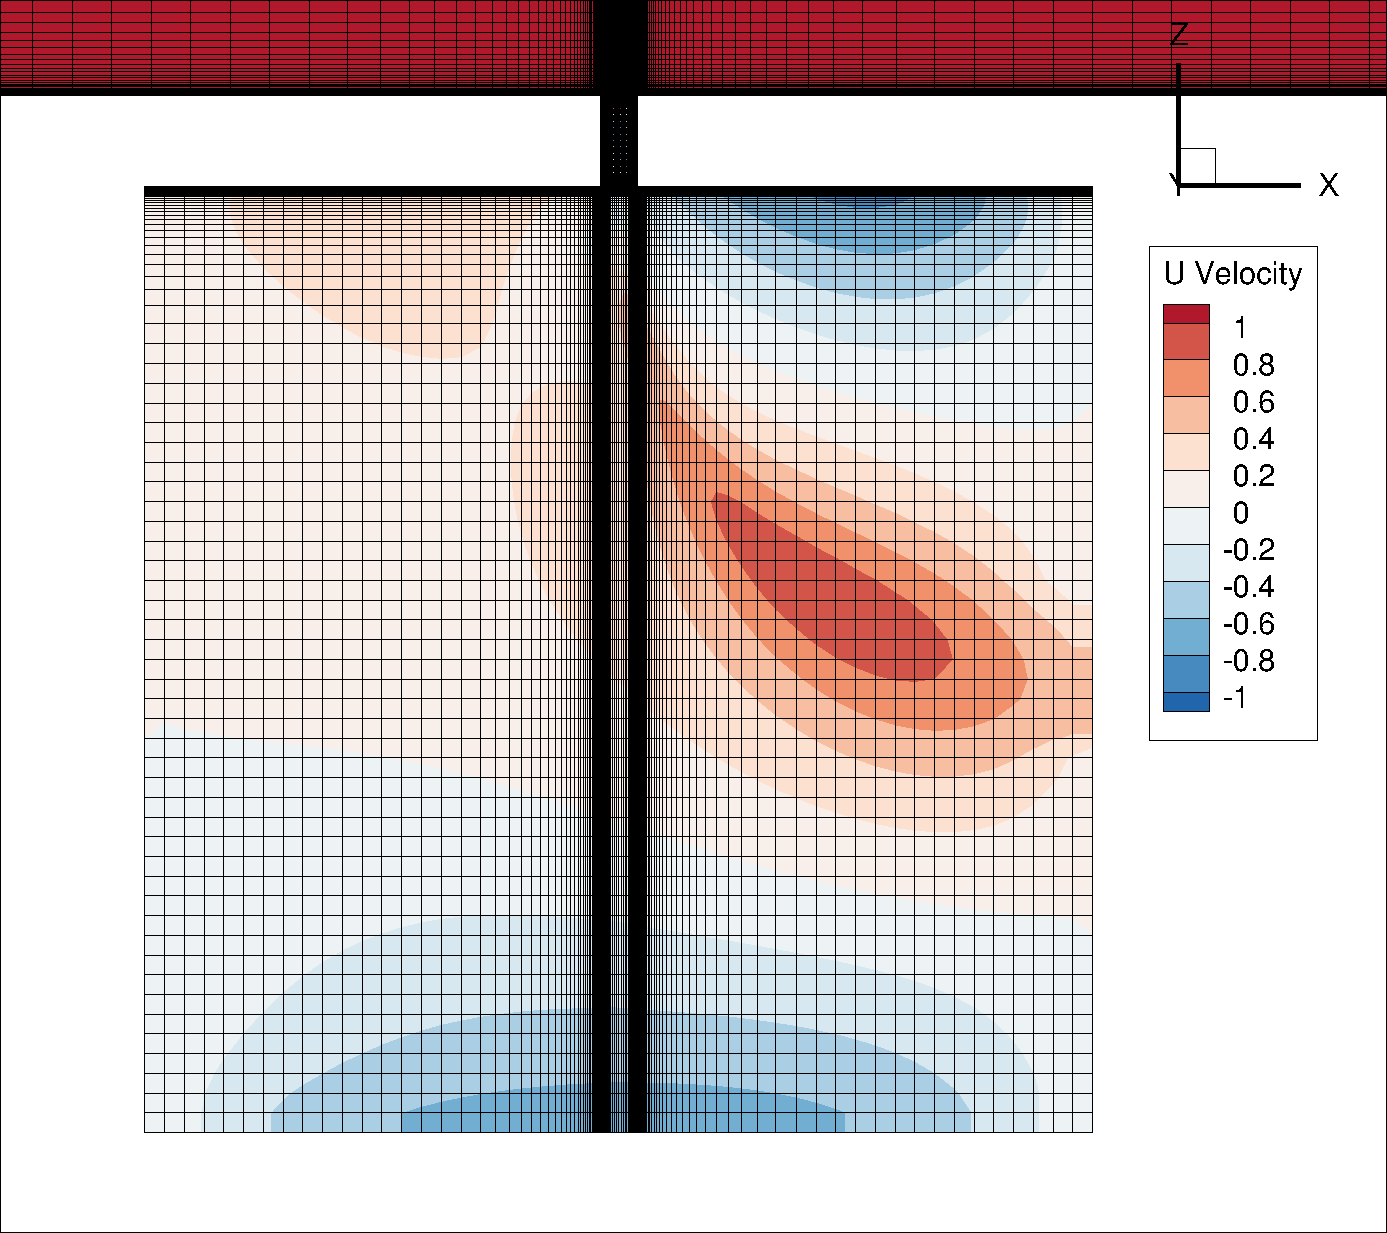
\includegraphics[width=1\linewidth]{2-2_grid.png}
%\end{subfigure}%
%\begin{subfigure}{.33\textwidth} \centering
%  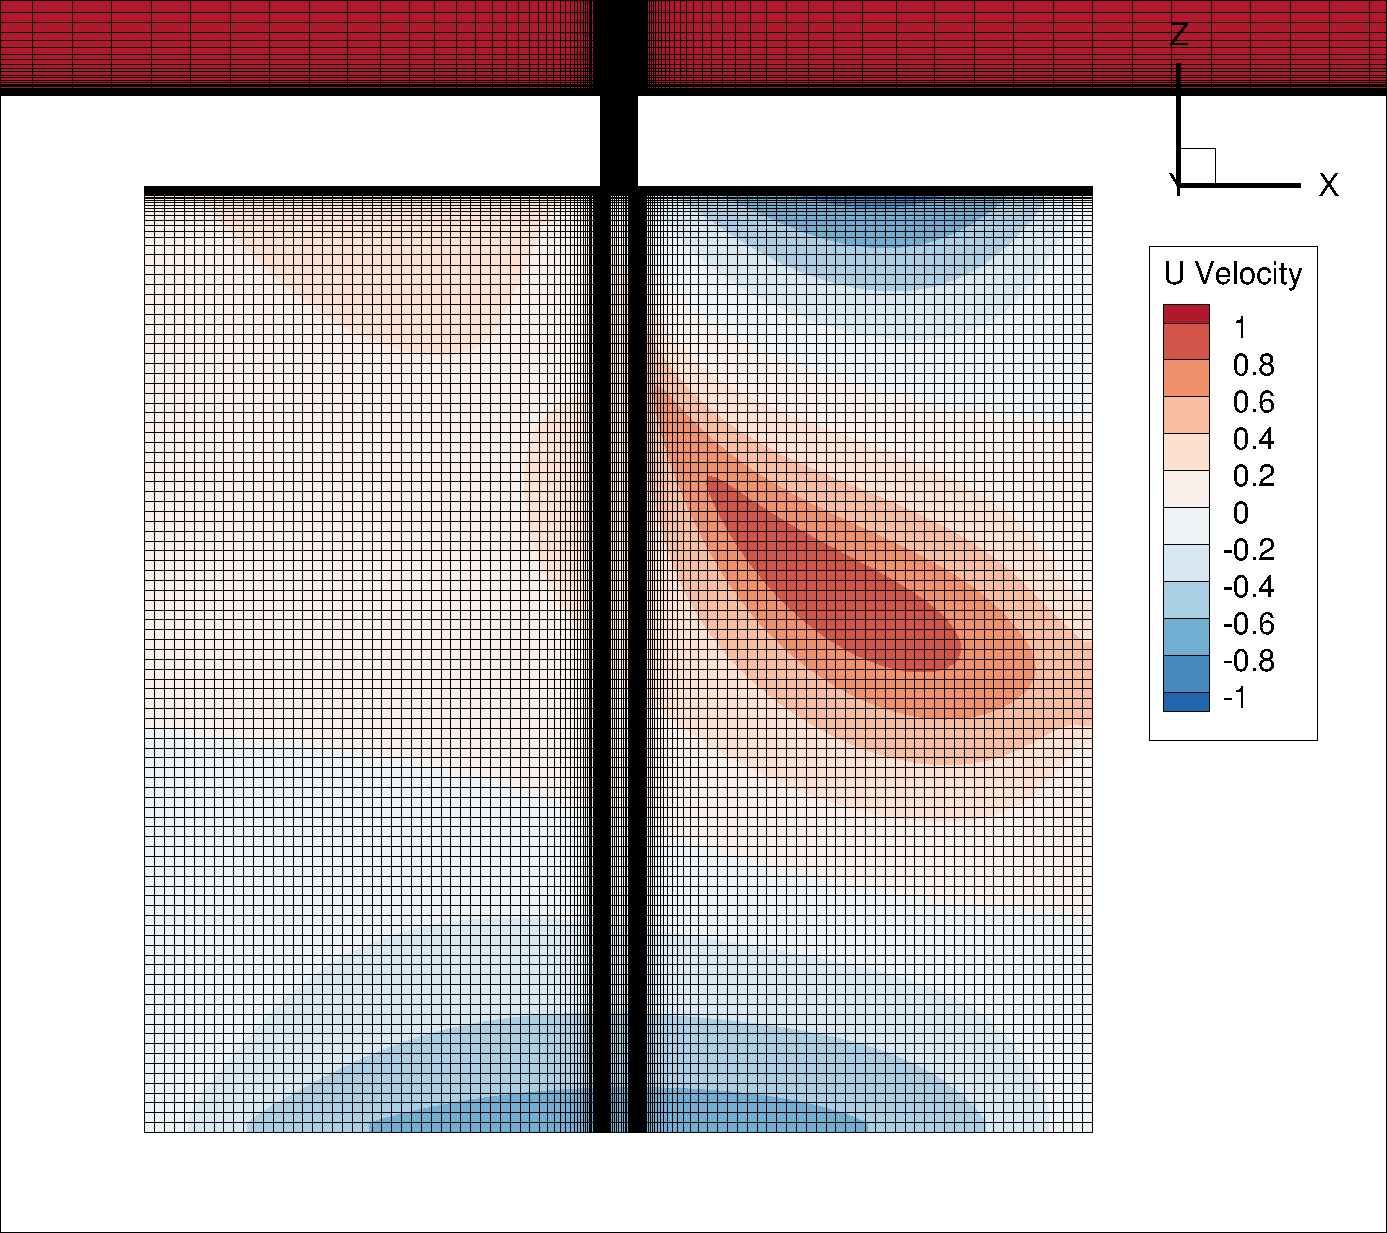
\includegraphics[width=1\linewidth]{2-3_grid.png}
%\end{subfigure}
%\begin{subfigure}{.33\textwidth} \centering
%  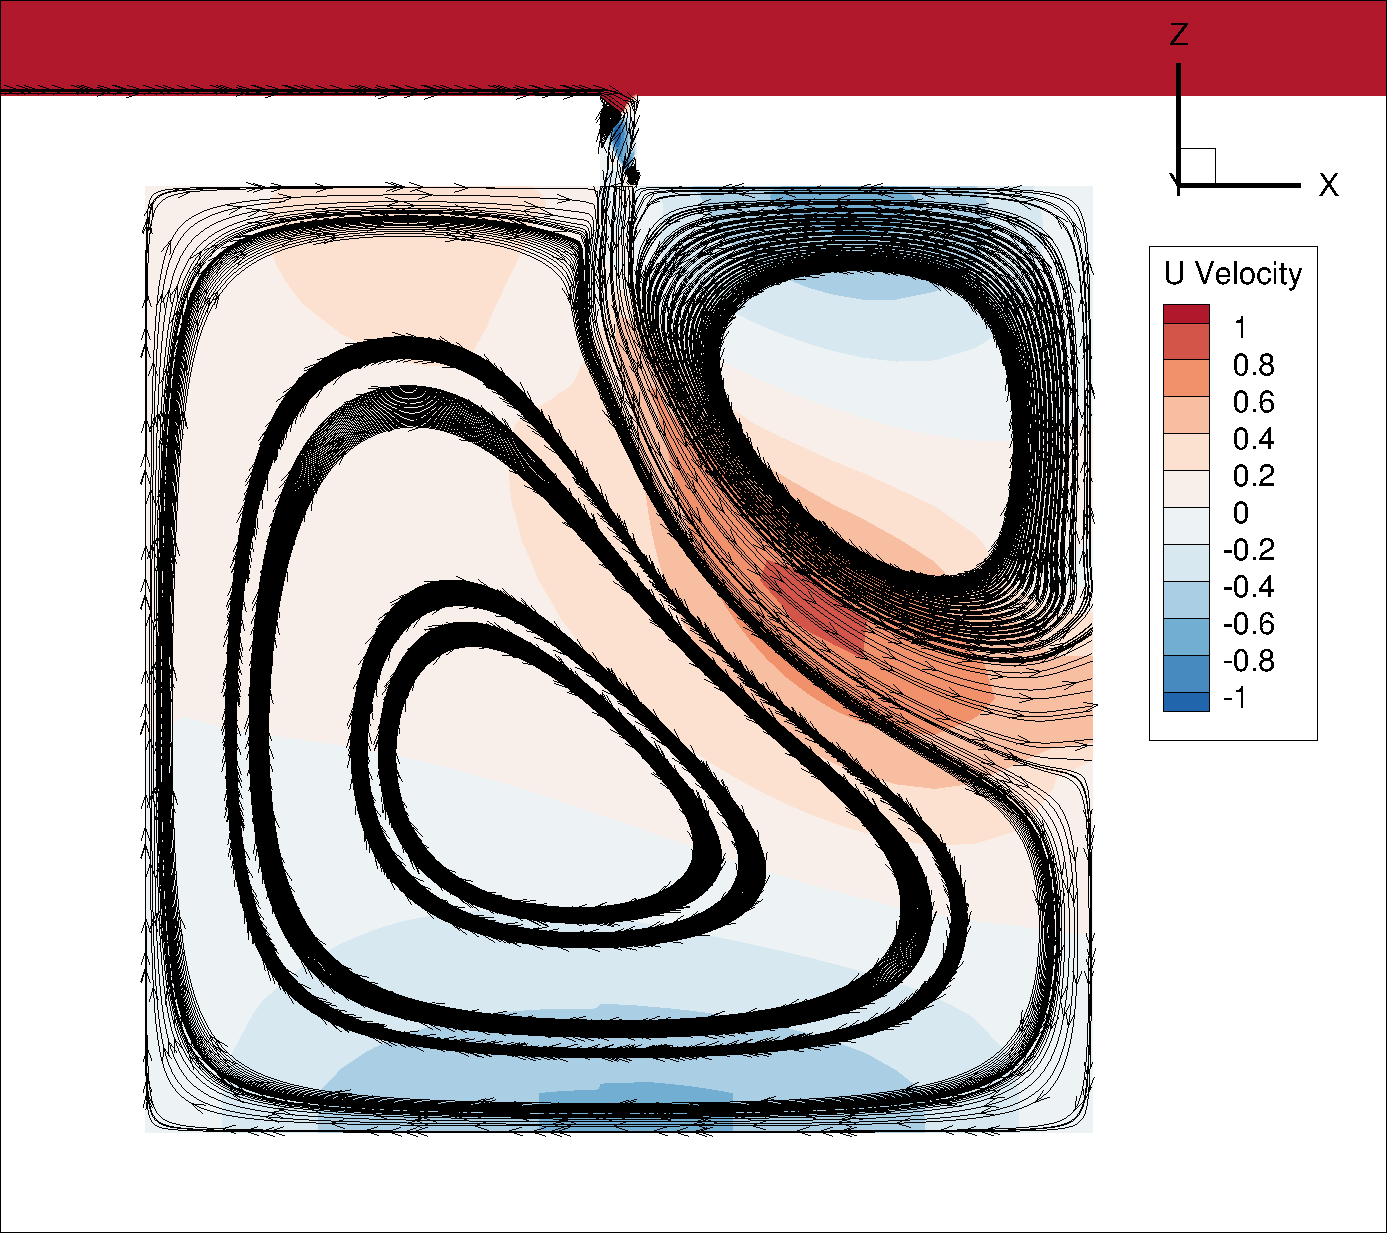
\includegraphics[width=1\linewidth]{2-1_streamlines.png}
%\end{subfigure}%
%\begin{subfigure}{.33\textwidth} \centering
%  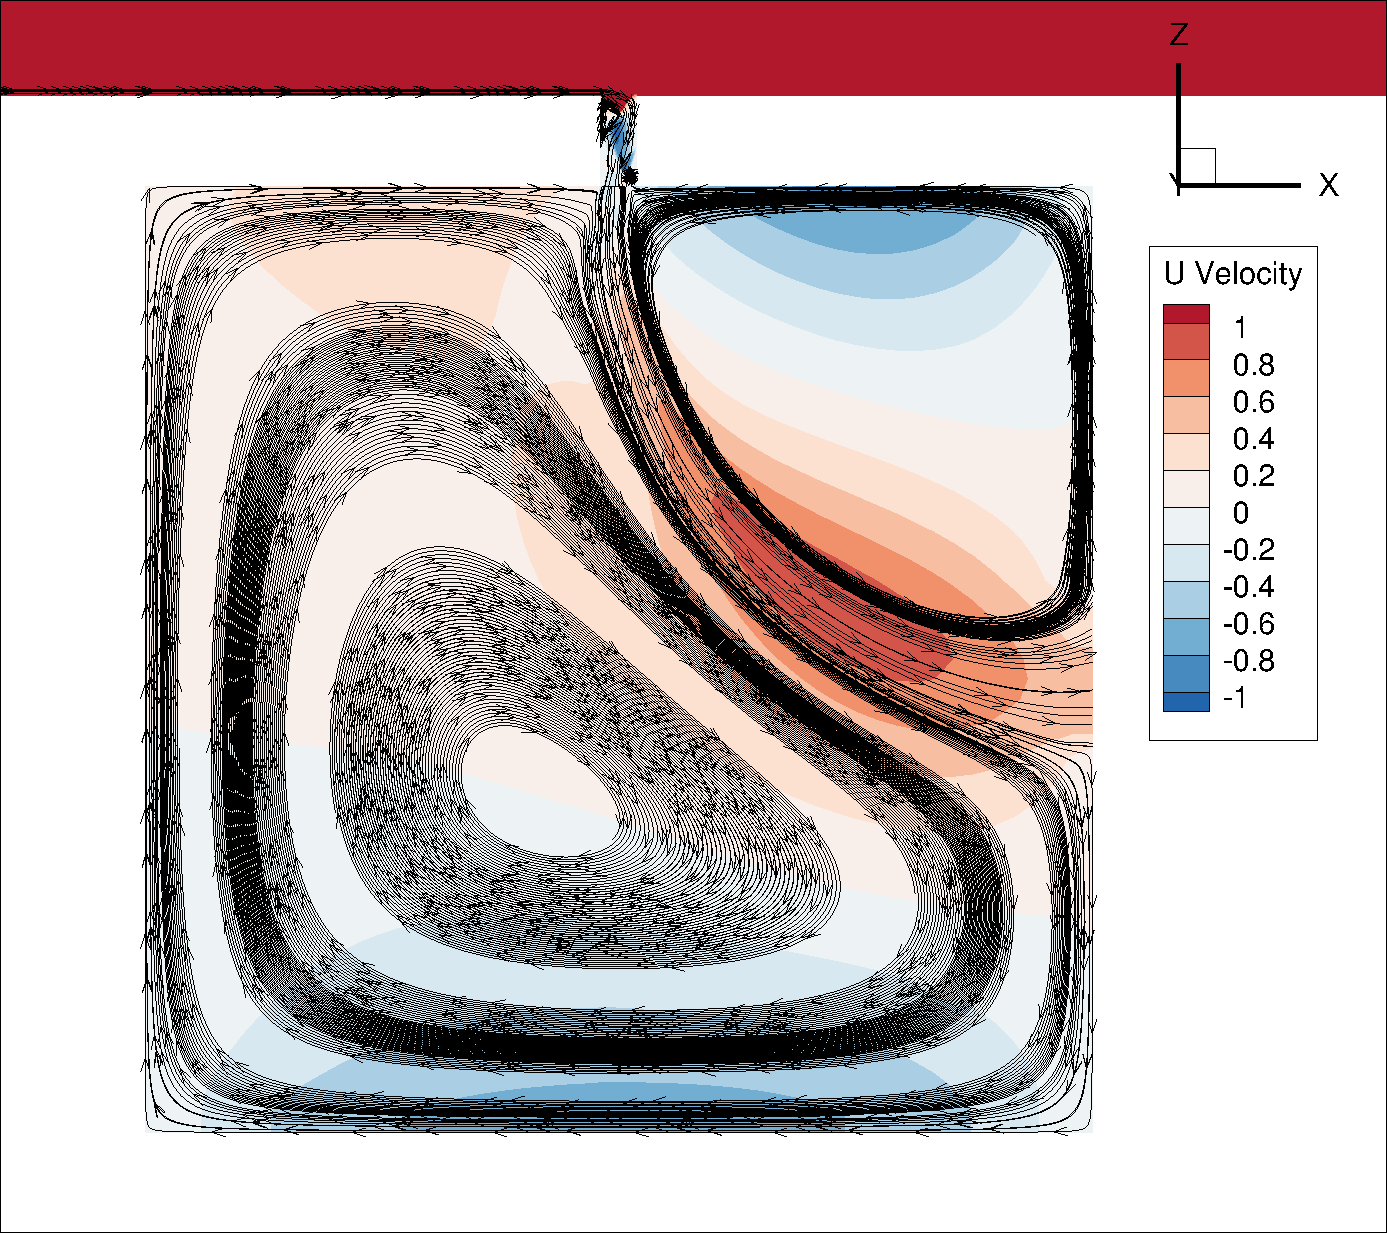
\includegraphics[width=1\linewidth]{2-2_streamlines.png}
%\end{subfigure}%
%\begin{subfigure}{.33\textwidth} \centering
%  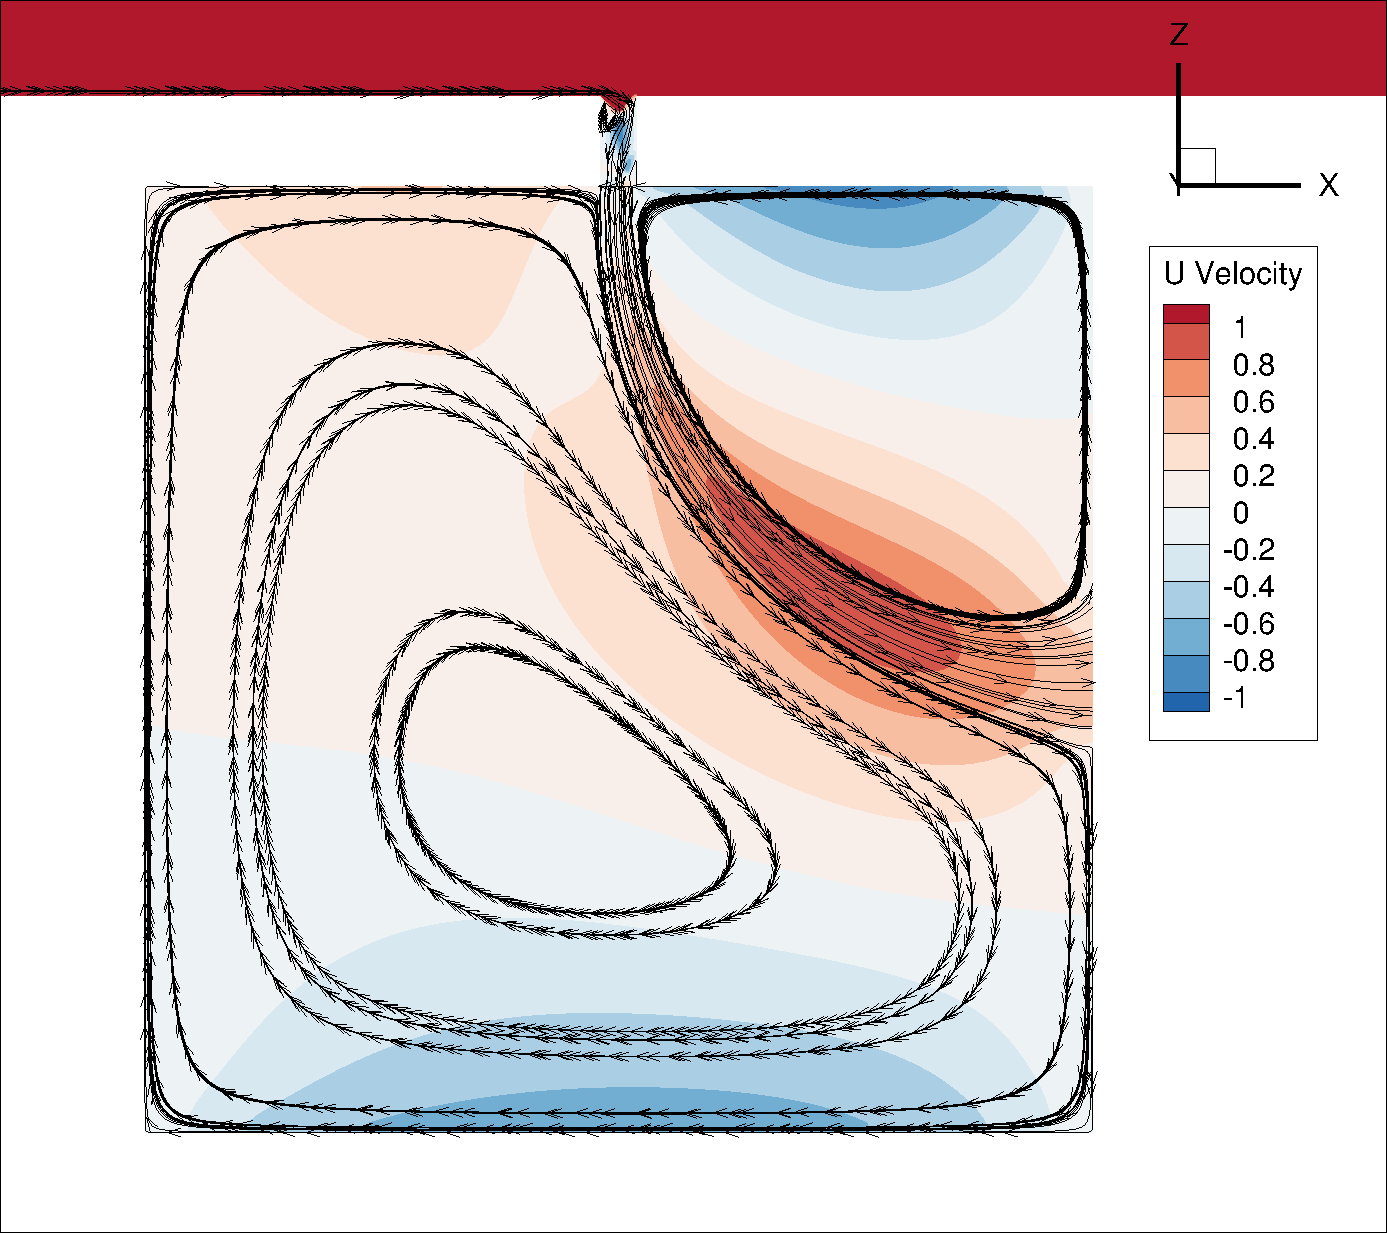
\includegraphics[width=1\linewidth]{2-3_streamlines.png}
%\end{subfigure}
%  \caption{Grid resolution study of the contours of u-velocity and streamlines for the medium patch}
%  \label{fig:med}
%\end{figure}

%\begin{figure}[H] \centering
%\begin{subfigure}{.33\textwidth} \centering
%  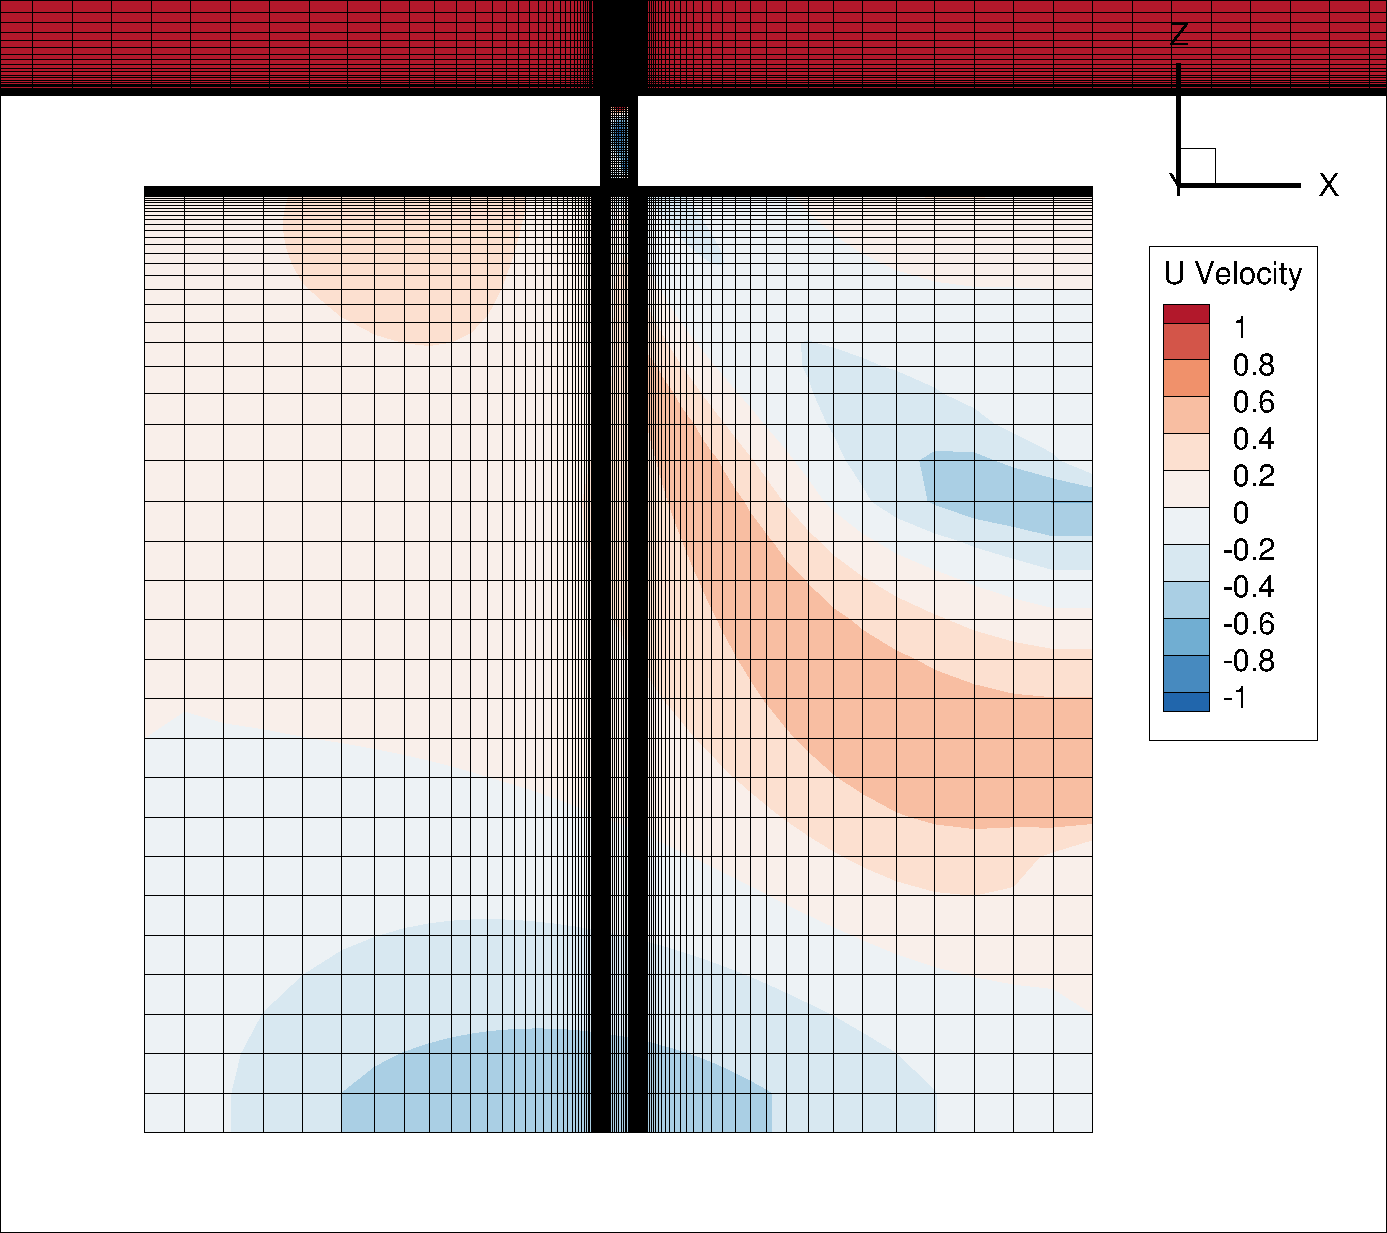
\includegraphics[width=1\linewidth]{3-1_grid.png}
%\end{subfigure}%
%\begin{subfigure}{.33\textwidth} \centering
%  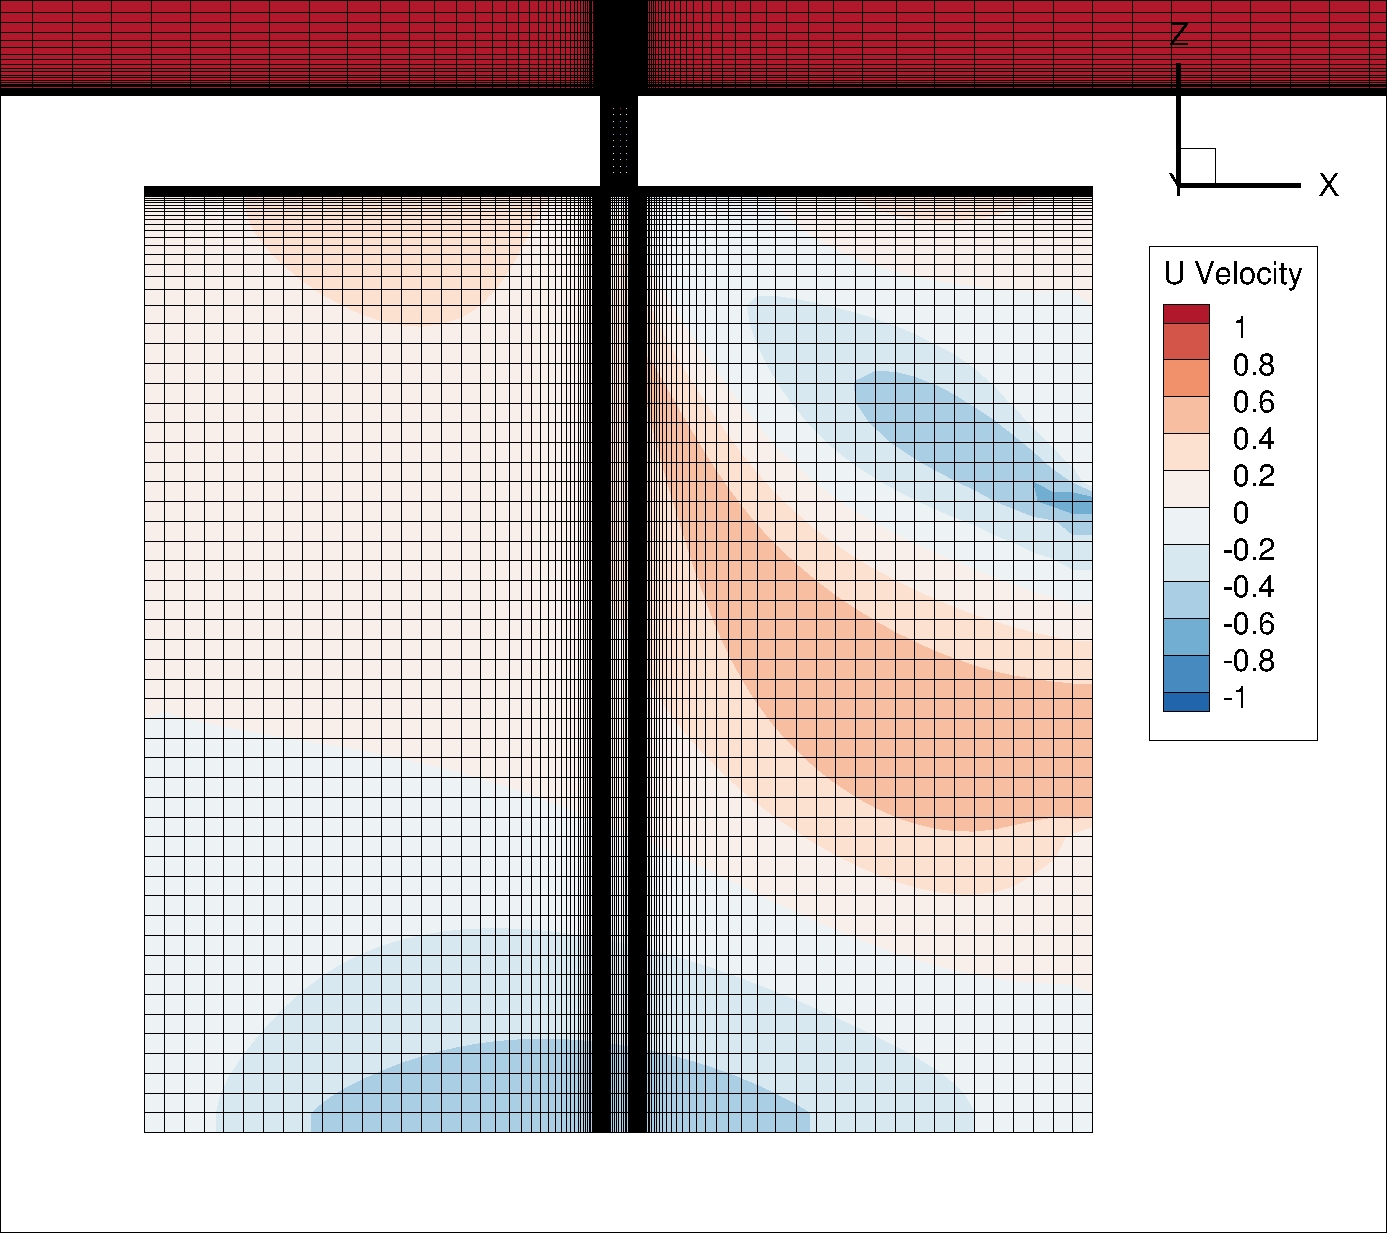
\includegraphics[width=1\linewidth]{3-2_grid.png}
%\end{subfigure}%
%\begin{subfigure}{.33\textwidth} \centering
%  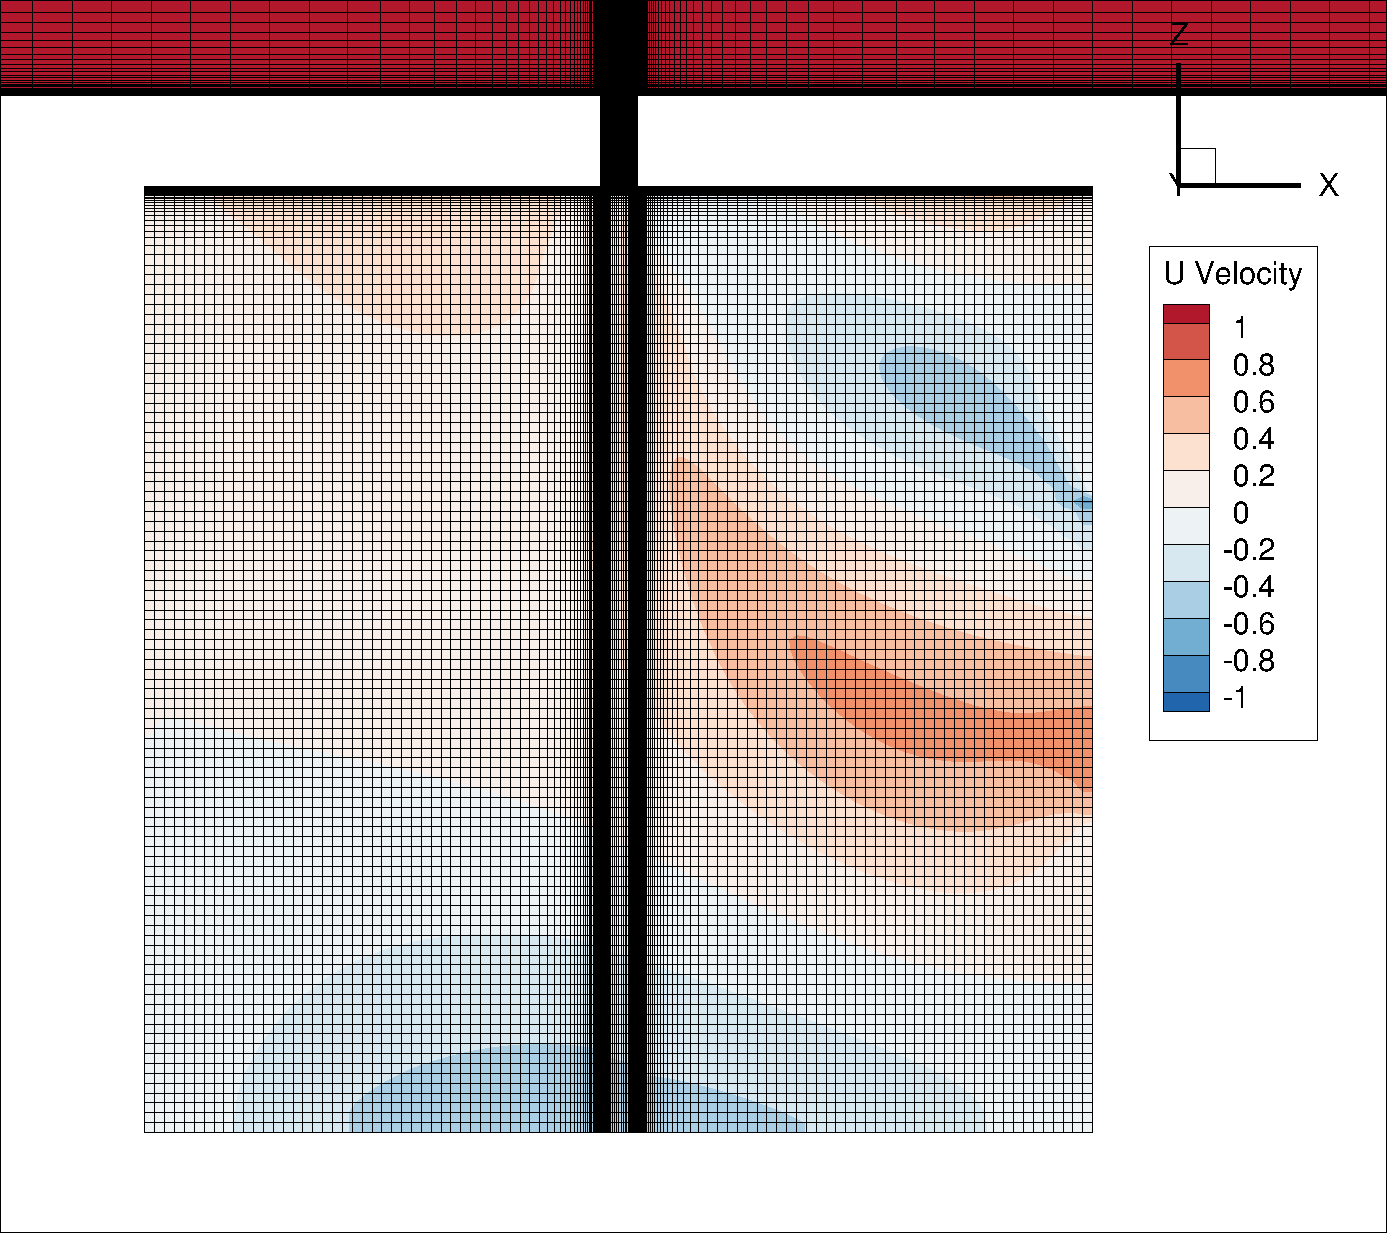
\includegraphics[width=1\linewidth]{3-3_grid.png}
%\end{subfigure}
%\begin{subfigure}{.33\textwidth} \centering
%  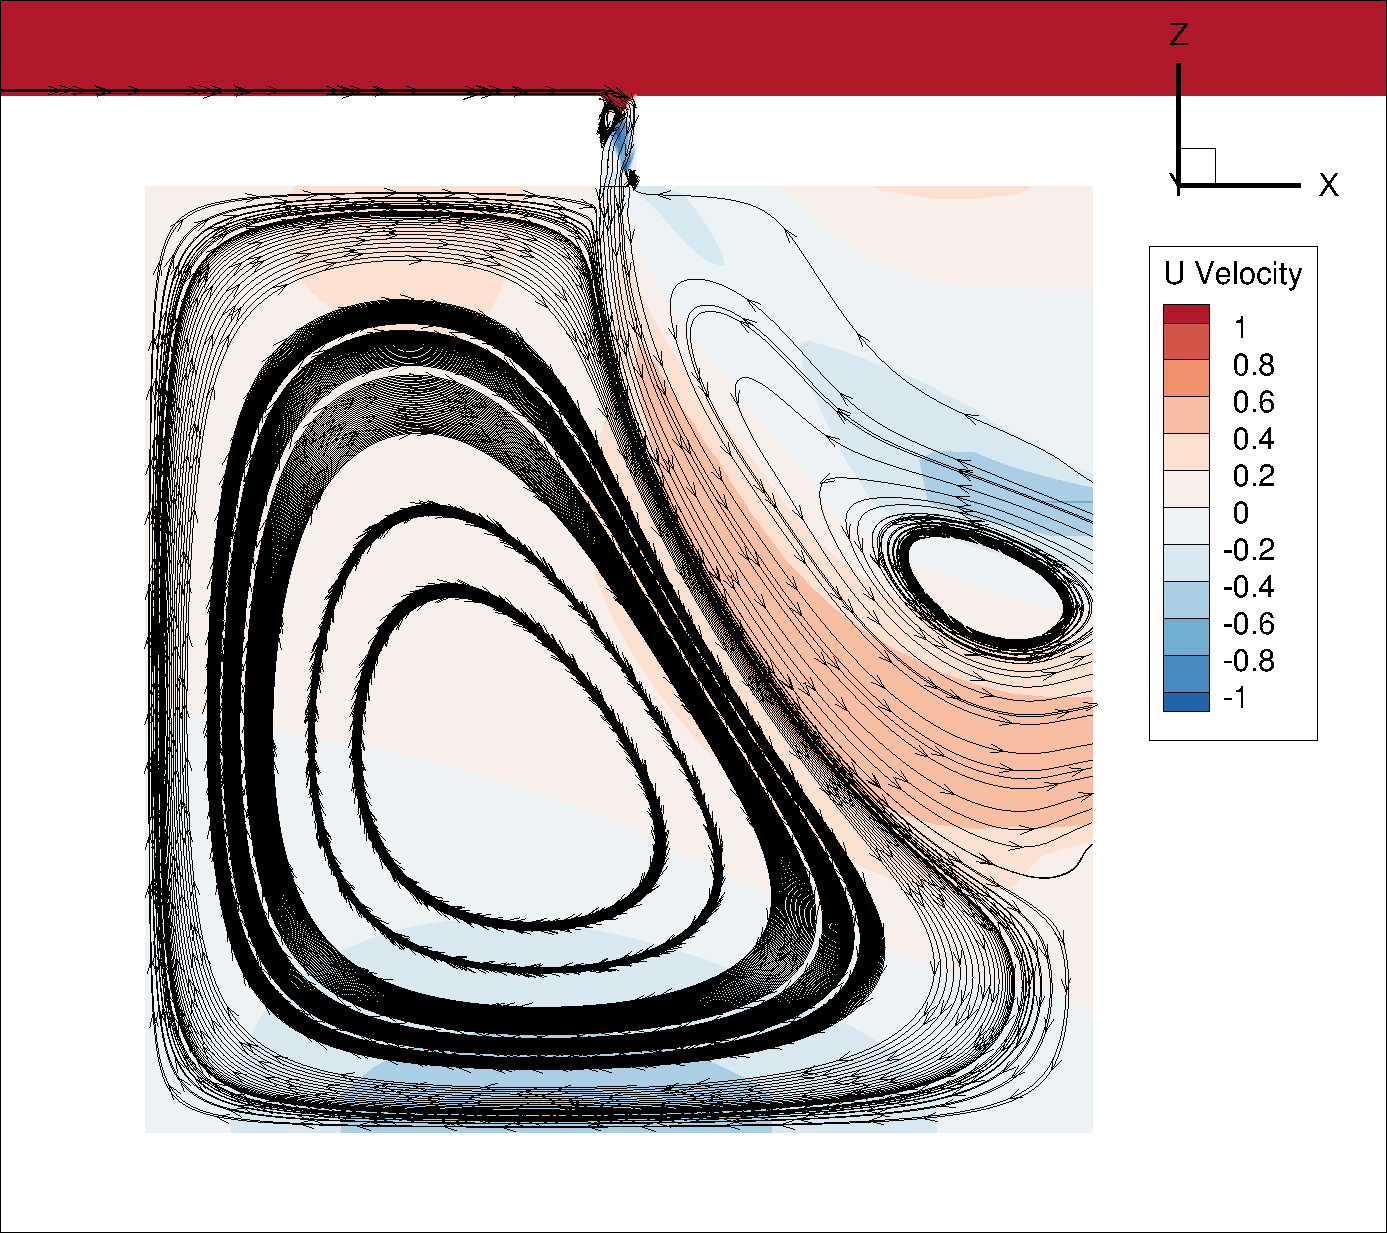
\includegraphics[width=1\linewidth]{3-1_streamlines.png}
%\end{subfigure}%
%\begin{subfigure}{.33\textwidth} \centering
%  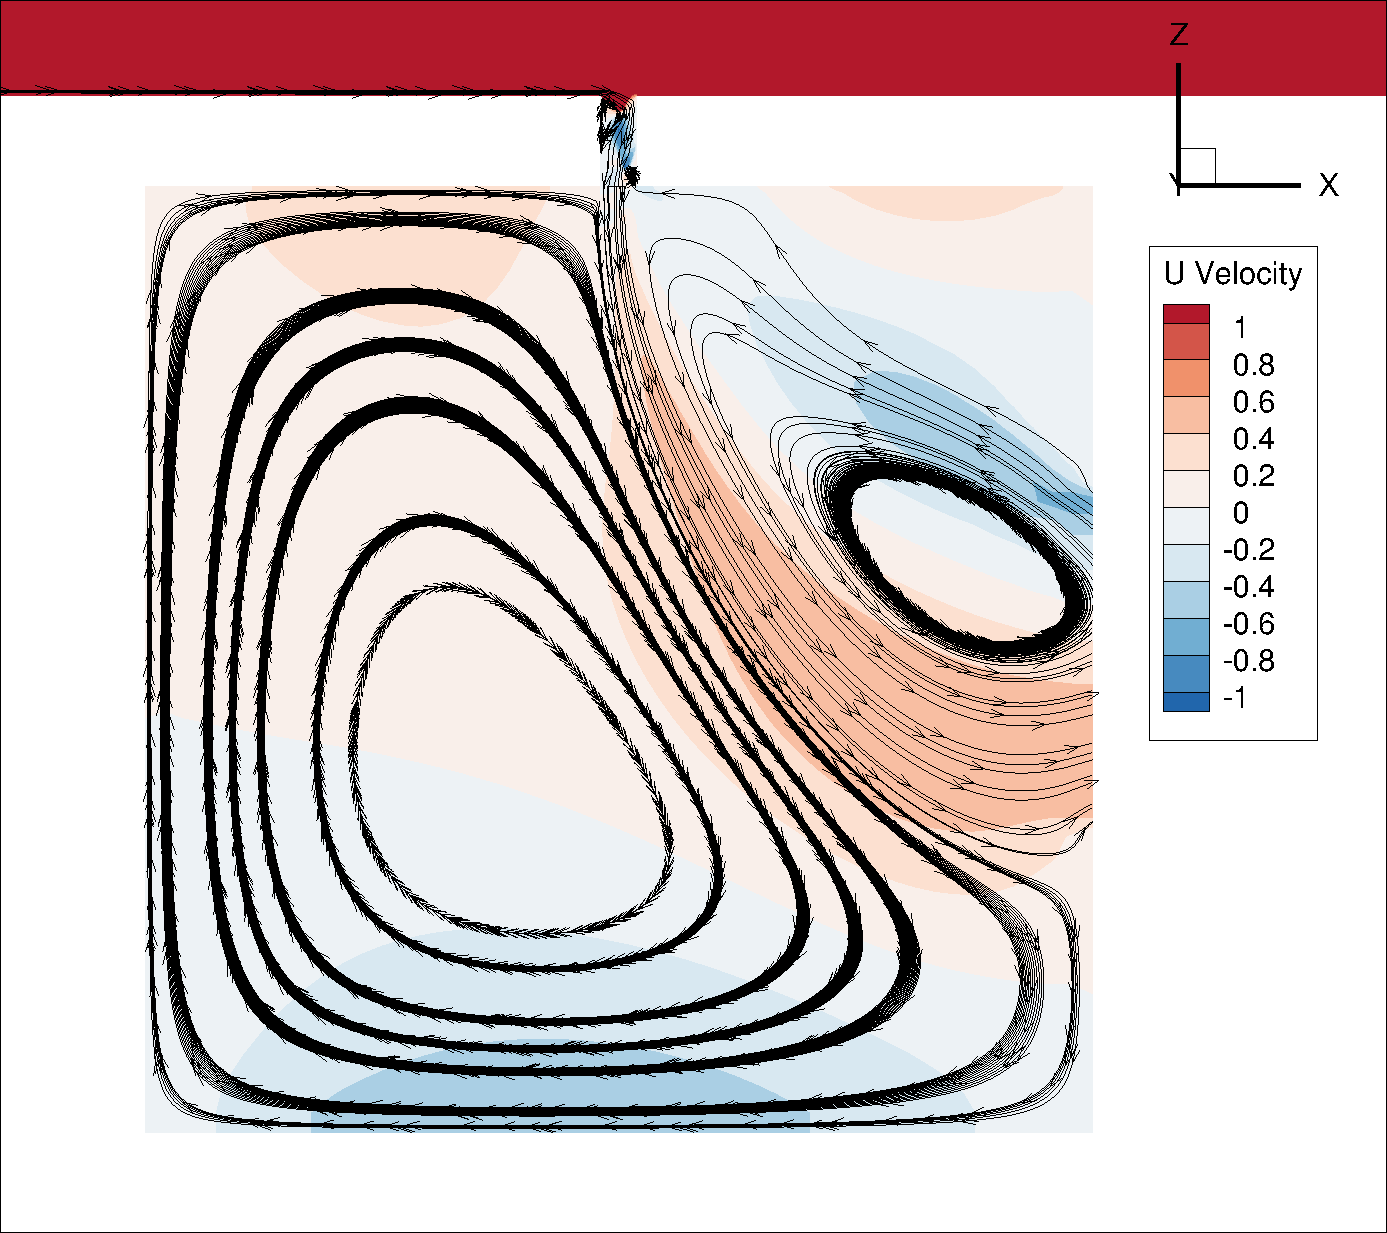
\includegraphics[width=1\linewidth]{3-2_streamlines.png}
%\end{subfigure}%
%\begin{subfigure}{.33\textwidth} \centering
%  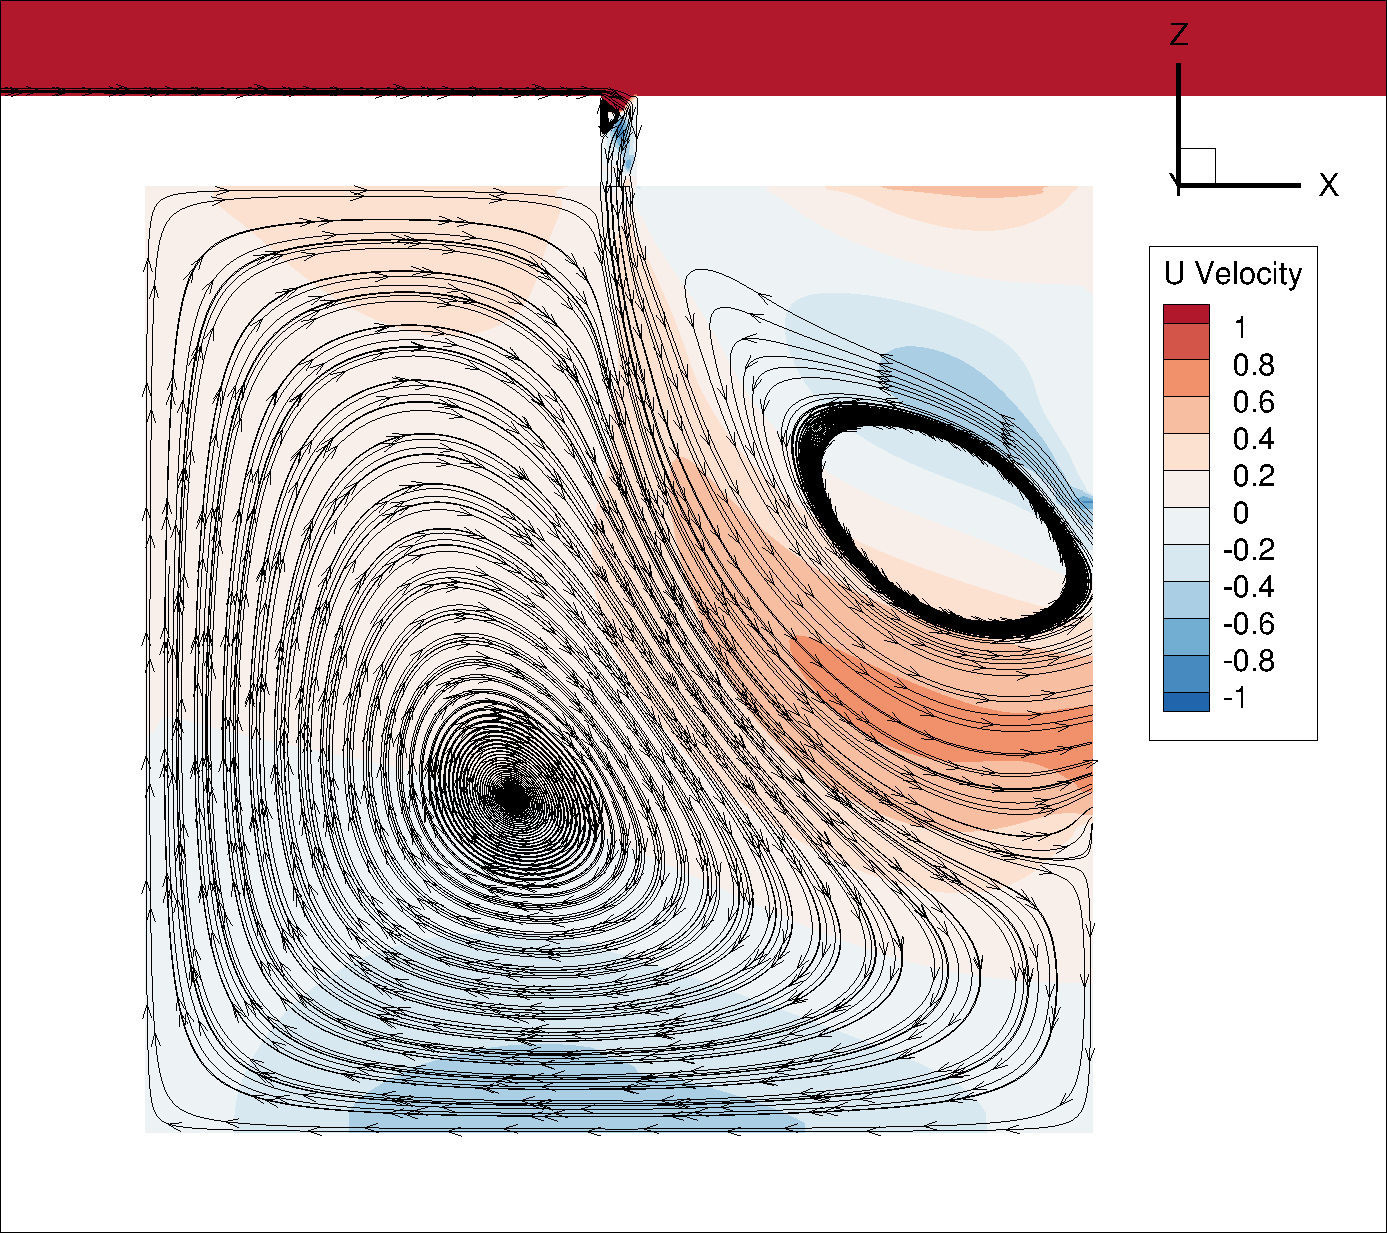
\includegraphics[width=1\linewidth]{3-3_streamlines.png}
%\end{subfigure}
%  \caption{Grid resolution study of the contours of u-velocity and streamlines for the large patch}
%  \label{fig:large}
%\end{figure}

%\begin{figure}[H] \centering
%  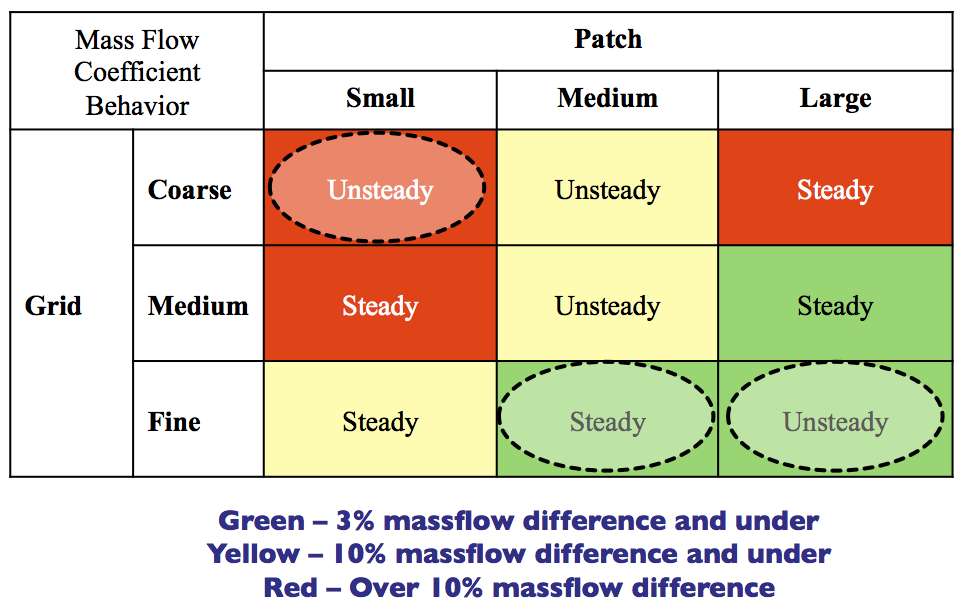
\includegraphics[width=.5\linewidth]{massflow_results.png}
%  \caption{Grid resolution and patch sizing study results where the circles represent cases that were more closely analyzed}
%  \label{fig:massflow_results}
%\end{figure}

The pressure at the plenum exit was varied to obtain 4 different pressure ratios and plotted against Slater's empirical relationship of experimental data \cite{dumArticle} as shown in \Cref{fig:slater}. We observe that the trends are similar but the data points do not lie on top of Slater's curve. This is most likely due to the fact that this simulation was performed in two dimensions, which would not accurately predict massflow of a three-dimensional hole.

%\begin{figure}[H] \centering
%  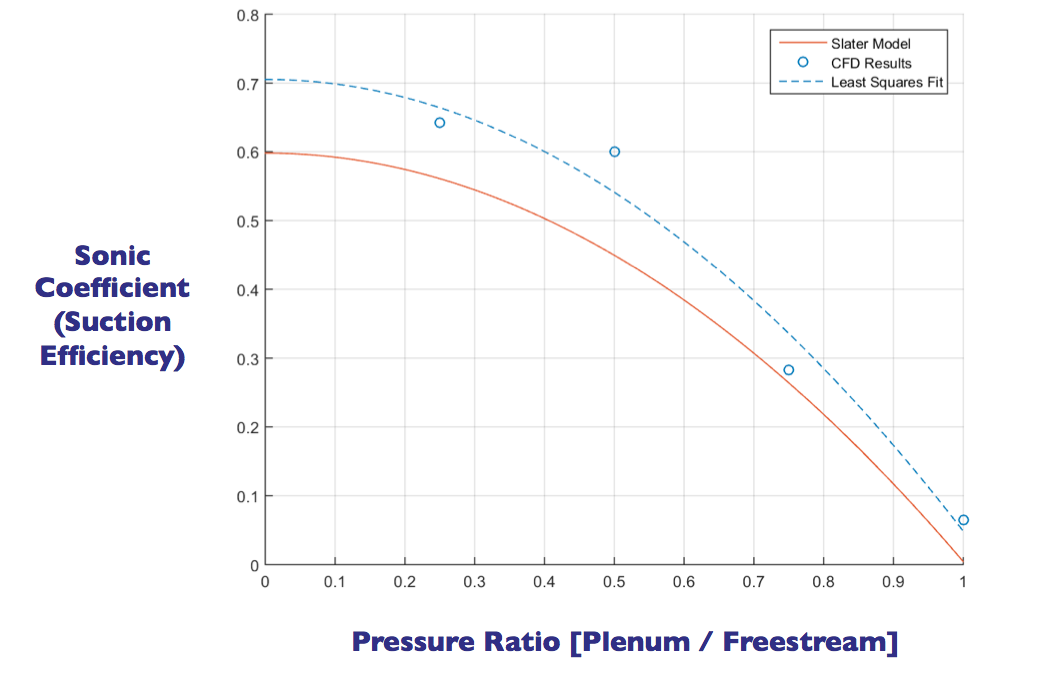
\includegraphics[width=.5\linewidth]{slater_model.png}
%  \caption{Comparison to experimental correlation}
%  \label{fig:slater}
%\end{figure}


% ------------------------------------------------------------------------- Shock Analysis


In order to properly study any upstream effects, an unsteady shock will need to be simulated. This could be challenging given the current constraints on the problem. Two canonical problems will be studied to produce the unsteady shock: a forward-facing step and a high-angle wedge. These scenarios will be run with URANS and a turbulence model study will be performed using 1- or 2-equation models to examine the effect of the choice of turbulence model in capturing unsteadiness in the shock. If turbulence model study does not produce the desired outcome, a Detached Eddy Simulation (DES) approach in two-dimension might be considered. Once the unsteady shock is generated, the shock motion will be analyzed and is expected to be random and noisy with no coherent frequency behavior.

Once the unsteady shock is properly modeled, bleed holes will be modeled in and an investigation will be performed on the change in flow structure in the bleed hole due to the presence of a shock. The quantities of bleed holes and their spacing relative to each other and relative to the shock will also be studied. Since this is a two-dimension simulation, only the streamwise spacing and location will be considered. This will aim to see how a desirable shock behavior can be obtained where desired behavior will be weighted favorably if the shock motion with bleed holes is predictable and weighted even more favorably if the shock motion becomes steady.




\section{Analysis}